%%%%%%%%%%%%%%%%%%%%%%%%%%%%%%%%%%%%%%%%%%%%%%%%%%%%%%%%%%%%%%%%%%%%%%%%%%%%%%%%
\documentclass[12pt]{extarticle}
%%%%%%%%%%%%%%%%%%%%%%%%%%%%%%%%%%%%%%%%%%%%%%%%%%%%%%%%%%%%%%%%%%%%%%%%%%%%%%%%
\usepackage{fontspec}
\usepackage{polyglossia}
\usepackage[a4paper, lmargin=30mm, rmargin=15mm, tmargin=20mm, bmargin=20mm]{geometry}
\usepackage{multirow}

\setdefaultlanguage{russian}
\setotherlanguage{english}

\defaultfontfeatures{Ligatures=TeX}

\setmainfont{Times New Roman}
\setmonofont{Courier New}
\setsansfont{Arial}

\newfontfamily\cyrillicfont{Times New Roman}
\newfontfamily\cyrillicfontsf{Arial}
\newfontfamily\cyrillicfonttt{Courier New}

\newfontfamily\englishfont{Times New Roman}
\newfontfamily\englishfontsf{Arial}
\newfontfamily\englishfonttt{Courier New}

\linespread{1.5}

\usepackage[backend=biber,
  bibencoding=utf8,
  sorting=none,
  style=gost-numeric,
  language=autobib,
  autolang=other,
  clearlang=true,
  defernumbers=true,
  sortcites=true,
  doi=true,
  isbn=true,
  ]{biblatex}

\usepackage[dvipsnames]{xcolor}

\definecolor{coolgrey}{rgb}{0.55, 0.57, 0.67} % This is the color of character in diagrams

\usepackage[
  hidelinks,
  colorlinks=true,
  linkcolor=Blue, % This is the color of table of contents and figure references
  citecolor=Blue, % This is the color of citations
  urlcolor=Blue % This is the colro of urls
]{hyperref}
\renewcommand{\UrlFont}{\small\rmfamily\tt}

\renewcommand\thesection{\arabic{section}}

\usepackage{amsfonts}
\usepackage{amsmath}

\usepackage{tikz} % This allows to make diagrams
\usetikzlibrary{arrows}
\usetikzlibrary{arrows.meta}
\usetikzlibrary{positioning}

\usepackage{caption}
\captionsetup[figure]{font=footnotesize}
\captionsetup[lstlisting]{font=footnotesize}

\usepackage{graphicx}
\graphicspath{ {./images/} } % This sets path to directory containing images.
\addto\captionsrussian{\renewcommand{\figurename}{Рисунок}} % This changes caption from 'Рис.' to 'Рисунок'.
\addto\captionsrussian{\renewcommand{\lstlistingname}{Листинг}} % This changes caption from 'Listing.' to 'Листинг'.

\usepackage{wrapfig}
\usepackage{subfigure}
\usepackage{subcaption}

\usepackage{titlesec}
% \setcounter{secnumdepth}{4}
% \setcounter{tocdepth}{4}

\usepackage{listings}
\usepackage{xcolor}
\usepackage{verbatimbox}

\definecolor{codegreen}{rgb}{0,0.6,0}
\definecolor{codegray}{rgb}{0.6,0.6,0.6}
\definecolor{codepurple}{rgb}{0.58,0,0.82}
\definecolor{backcolour}{rgb}{0.95,0.95,0.95}

\lstdefinestyle{cppstyle}{
  % backgroundcolor=\color{backcolour},
  commentstyle=\color{codegreen},
  keywordstyle=\color{magenta},
  numberstyle=\tiny\color{codegray},
  stringstyle=\color{codepurple},
  basicstyle=\ttfamily\scriptsize,
  % basicstyle=\scriptsize,
  breakatwhitespace=false,
  breaklines=true,
  captionpos=b,
  keepspaces=true,
  numbers=left,
  numbersep=5pt,
  showspaces=false,
  showstringspaces=false,
  showtabs=false,
  tabsize=2,
  % frame=tB
}

\lstdefinestyle{pseudocodestyle}{
  mathescape=true,
  frame=tB,
  numbers=left, 
  % numberstyle=\tiny,
  numberstyle=\tiny\color{codegray},
  numbersep=5pt,
  basicstyle=\scriptsize,
  keywordstyle=\color{black}\bfseries,
  keywords={,return, function, in, if, else, while, true, false, and, not} %add the keywords you want, or load a language as Rubens explains in his comment above.
  numbers=left,
  captionpos=b,
  breakatwhitespace=false
}

% \lstset{style=mystyle}

\usepackage{regexpatch}% http://ctan.org/pkg/regexpatch
\usepackage{listings}% http://ctan.org/pkg/listings
\makeatletter

\newcommand{\lstlistcplusplusname}{List of C++}
\lst@UserCommand\lstlistofcplusplus{\bgroup
    \let\contentsname\lstlistcplusplusname
    \let\lst@temp\@starttoc \def\@starttoc##1{\lst@temp{loc}}%
    \tableofcontents \egroup}
\lstnewenvironment{cpp}[1][]{%
  \renewcommand{\lstlistingname}{C++ Листинг}%
  \xpatchcmd*{\lst@MakeCaption}{lol}{loc}{}{}%
  \lstset{style=cppstyle, language=C++,#1}}
  {}

\newcommand{\lstlistpseudocodename}{List of Pseudocode}
\lst@UserCommand\lstlistofpseudocode{\bgroup
    \let\contentsname\lstlistpseudocodename
    \let\lst@temp\@starttoc \def\@starttoc##1{\lst@temp{lop}}%
    \tableofcontents \egroup}
\lstnewenvironment{pseudocode}[2][]{%
  \renewcommand{\lstlistingname}{Алгоритм}%
  \xpatchcmd*{\lst@MakeCaption}{lol}{lop}{}{}%
  \lstset{style=pseudocodestyle,#1}}
  {}
\makeatother

%%%%%%%%%%%%%%%%%%%%%%%%%%%%%%%%%%%%%%%%%%%%%%%%%%%%%%%%%%%%%%%%%%%%%%%%%%%%%%%%
\addbibresource{biblio/bibliography.bib}
%%%%%%%%%%%%%%%%%%%%%%%%%%%%%%%%%%%%%%%%%%%%%%%%%%%%%%%%%%%%%%%%%%%%%%%%%%%%%%%%
\renewcommand*{\maketitle}{
\begin{titlepage}
  \begin{center}
    \linespread{1}
    \small
    Федеральное государственное автономное образовательное учреждение\break высшего образования\par
    <<Московский физико-технический институт \break (национальный исследовательский университет)>>\par
    Физтех-школа Прикладной Математики и Информатики\par
    Центр обучения проектированию и разработке игр\par
  \end{center}
%
  {
    \small
    {\bf Направление подготовки / специальность}: 09.03.01 Информатика и вычислительная техника\newline
    {\bf Направленность (профиль) подготовки}: Компьютерные науки и инженерия
  }
%
  {
    \topskip0pt
    \vspace*{\fill}
    \begin{center}
      {\bf\Large ИМПЛЕМЕНТАЦИЯ И ПРИМЕНЕНИЕ КАДРОВЫХ ГРАФОВ В РЕНДЕРИНГЕ РЕАЛЬНОГО ВРЕМЕНИ}\par(бакалаврская работа)
    \end{center}
    \vspace*{\fill}
  }
%
  \hfill
  \begin{minipage}[t]{8cm}
    {\bf Студент: \newline}
    Мочалов Никита Андреевич\newline
    \vspace{-3mm}
    \rule{8cm}{0.15mm}
    \centerline{\scriptsize\it (подпись студента)}\newline
%
    {\bf Научный руководитель: \newline}
    Лесовой Алексей Игоревич\newline
    \vspace{-3mm}
    \rule{8cm}{0.15mm}
    \centerline{\scriptsize\it (подпись научного руководителя)}
  \end{minipage}

  \vspace*{\fill}
  \begin{center}
    Москва 2024
  \end{center}
\end{titlepage}
}
%%%%%%%%%%%%%%%%%%%%%%%%%%%%%%%%%%%%%%%%%%%%%%%%%%%%%%%%%%%%%%%%%%%%%%%%%%%%%%%%
\begin{document}
%%%%%%%%%%%%%%%%%%%%%%%%%%%%%%%%%%%%%%%%%%%%%%%%%%%%%%%%%%%%%%%%%%%%%%%%%%%%%%%%
\maketitle
\newpage
\setcounter{page}{2}
\vspace*{\fill}
\begin{abstract}

Данная работа посвящена разработке кадрового графа и исследованию его связи со слоем абстракции над графическими API (Render Hardware Interface). Было предложено внедрить данный механизм непосредственно в слой абстракции. В результате работы была написана эффективная имплементация кадрового графа с использованием современного графического API Vulkan. Кроме того, был спроектирован и реализован высокоуровневый рендерер в качестве доказательства практической применимости выбранного дизайна.

% Данная работа посвящена разработке кадрового графа. Было предложено внедрить данный механизм непосредственно в слой абстракции над графическими API (Render Hardware Interface). Такое решение позволяет использовать уникальные возможности каждого API с целью повышения производительности. В результате работы была написана эффективная имплементация кадрового графа с использованием современного графического API Vulkan. Кроме того, был спроектирован и реализован высокоуровневый рендерер в качестве доказательства практической применимости выбранного дизайна.

% Данная работа посвящена разработке кадрового графа и исследованию его связи с абстракцией Render Hardware Interface. Был предложен способ внедрения данного механизма напрямую в RHI, а также разобраны преимущества и недостатки этого подхода. В результате работы была написана эффективная имплементация кадрового графа, позволяющего утилизировать возможности нескольких командных очередей, с использованием современного графического API "Vulkan", а также был спроектирован и реализован высокоуровневый рендерер в качестве доказательства валидности дизайна.

% Данная работа посвящена разработке кадрового графа. Был предложен способ внедрения данного механизма непосредственно в слой абстракции графических API (Render Hardware Interface). В результате работы была написана эффективная имплементация кадрового графа, позволяющего утилизировать возможности нескольких командных очередей, с использованием современного графического API "Vulkan". Помимо этого был спроектирован и реализован высокоуровневый рендерер в качестве доказательства валидности дизайна.
\end{abstract}
\vspace*{\fill}
\newpage
\tableofcontents
\newpage
\section{Введение}
% Как таковое, понятие «игровой движок» появилось в середине 90-х годов прошлого века с выходом \textit{Doom Engine} в 1995 году. Данный продукт заложил основные идеи выявления ключевых переиспользуемых модулей, независимых от конкретной игры, с целью ускорить итерационность разработки новых игр. Первые такие движки были спроектированы для конкретных жанров, или даже конкретной игровой серии (как в случае с \textit{Doom Engine}). Однако за последние несколько десятилетий концепция игрового движка сильно преобразовалась. Ключевым изменением стало стремление к созданию движков, позволяющих создавать игры произвольных жанров и c разнообразными художественными стилями. Данная тенденция к созданию слоев абстракций не является уникальной для индустрии видеоигр и может наблюдаться во всех сферах разработки. Отличием же игровых движков от большинства других программных продуктов является необходимость хорошей производительности в реальном времени, что ограничивает разработчиков в абстрагировании различных частей движка, заставляя идти на компромисс между общностью, удобством и производительностью.

% Современные игровые движки должны поддерживать разные виды устройств, операционные системы и зачастую немалый диапазон аппаратного обеспечения. Добавив к этому большое количество подсистем, инструментов, а также возможность написания игр произвольных стилей и жанров, получится огромная комбинаторная сложность. Именно из-за этого написание нового игрового движка в современном мире довольно комплексная задача, требующая немалого количества специалистов, много времени и бюджета. Это привело к тому, что крупные движки вынуждены вводить комиссии для разработчиков за каждую проданную копию игры. В последние годы из-за чрезмерной комплексности движков и тяжелой комиссионной политики, разработчики игр стали задумываться о переходе на относительно новые движки с открытым исходным кодом, что особенно распространяется на некрупные игровые студии, которые не в состоянии отдавать большой процент от продаж и нанимать высококвалифицированных разработчиков, способных модифицировать крупные движки под проектные нужды.

% С ростом производительности аппаратного обеспечения, появлением новых технологий и непрерывным увеличением масштабов современных игровых проектов архитектурные паттерны проектирования движков потерпели значимые изменения и развитие. Однако ввиду комплексности, о которой было упомянуто ранее, крупные движки неспособны быстро реализовывать новые подходы, а в некоторых случаях не в состоянии реализовать их вообще, ведь они могут потребовать полного перепланирования всего движка.

% Целью данной работы таким образом является исследование современных подходов к архитектуре игровых движков, а также базовая имплементация некоторых из них.

% Рендеринг реального времени значительно изменился за последние несколько десятилетий благодаря достижениям в аппаратных возможностях и программных решениях. Отрисовка современных видеоигр состоит из большого количества вычислений, которые еще недавно казались недостижимыми в интерактивных приложениях. С ростом комплексности рендеринга и особенно с появлением современных графических программных интерфейсов, таких как Vulkan, Directx 12 и Metal, в индустрии появилась необходимость в новом архитектурном решении декомпозиции рендеринга. Одним из таких решений являются кадровые графы.

% Кадровый граф является одним из способов организации работы на GPU и представляет из себя ориентированный ациклический граф, где вершины являются вычислительными задачами, а ребра между ними задают зависимости в порядке исполнения. Декомпозиция рендеринга на отдельные единицы исполнения упрощает процесс разработки новых графических эффектов, а полный граф дает глобальное представление о процессе отрисовки одного кадра (или же части кадра), что часто полезно при анализе производительности и отладке приложений. Важно заметить, что кадровые графы являются не только архитектурным решением структурирования рендеринга, но и мощным инструментом оптимизации. Обладание полной картиной кадра еще до момента исполнения позволяет (автоматически) утилизировать современные функции графических API, таких как, например, использование нескольких командных очередей, многопоточная запись командных буферов и др.


% \subsection{Базовые определения}
% Провести границу между понятиями «видеоигра» и «игровой движок» не всегда можно однозначно, и для каждого конкретного случая она будет разной. Однако для конструктивного анализа важно все же зафиксировать четкое разграничение между этими понятиями. Важно заметить, что в виду специфики данной работы дальше приводятся определения с инженерной точки зрения.

% Прежде всего, \textit{видеоигра}, или же просто \textit{игра}, как программный продукт, представляет собой синергетическое сочетание содержательной части (контента) и логической части (программной логики), создающее интерактивную виртуальную среду.

% Под \textit{игровым движком} понимается комплекс программных модулей, обеспечивающий реализацию основных функций игры, таких как графика, организация игрового мира, работа с ресурсами, физика, звук, работа с сетью и т.д. Он представляет собой набор библиотек, который позволяет разработчикам создавать игры различных жанров и уровней комплексности для потенциально нескольких платформ. Игровые движки значительно упрощают и ускоряют процесс разработки, предоставляя готовые решения для многих задач. Однако важно заметить, что видеоигры не обязаны разрабатываться на основе какого-либо игрового движка.

% Наконец, \textit{игровой редактор}, или просто \textit{редактор} -- программа с графическим интерфейсом, предоставляющая возможность создавать контент игры, утилизируя игровой движок. Это программное обеспечение позволяет разработчикам и дизайнерам реализовывать творческие идеи, не погружаясь полностью в технические детали реализации движка. Оптимальный дизайн игрового редактора способствует повышению эффективности разработки игр и сокращению времени, необходимого для воплощения итеративных изменений в игровых проектах. Часто под движком понимают именно редактор, однако с инженерной точки зрения, это принципиально разные понятия, особенно, если рассматривать движки, в принципе не имеющие редактора.



% % \subsection{Высокоуровневый обзор модулей}
% Существует принципиально две различные компоненты движка -- программный комплекс исполнения (\textit{engine runtime}) и набор инструментов разработки (\textit{tool suit}), второе часто представляет из себя в совокупности игровой редактор.

% % \subsubsection{Инструменты разработки/редактор}
% Набор инструментов разработки -- инструменты для создании и модификации контента игры. Эти инструменты предоставляют разработчикам интерфейсы и функции для работы с различными аспектами игры, включая графику, звук, анимацию и игровой процесс. Чаще всего эти инструменты являются частью игрового редактора. Примерами инструментов могут послужить:

% \begin{itemize}
%     \item \textit{Редактор уровней} позволяет дизайнерам создавать и редактировать игровые уровни, размещать объекты и настраивать игровые события.
%     \item \textit{UI редактор} используется для разработки и настройки элементов внутриигрового пользовательского интерфейса.
%     \item \textit{Редактор ассетов} используется для импорта, настройки и управления различными видами игрового контента.
%     \item \textit{Инструменты анимации} обеспечивают создание и настройку анимаций для персонажей и объектов.
%     \item \textit{Инструменты сборки} позволяют собирать финальный игровой продукт для целевых платформ.
% \end{itemize}

% % \subsubsection{Модули исполнения}
% Программный комплекс исполнения (или ядро движка) отвечает за запуск и функционирование игры в режиме реального времени. Модули исполнения обрабатывают ввод, обновляют игровую логику, рендеринг мира, воспроизведение звука и многое другое. Именно эта часть игрового движка рассматривается в данной работе.

% Как и в большинстве больших программных систем, движок можно разделить на несколько слоев, где более высокоуровневые слои используют низкоуровневые.



% \subsection{Разбор существующих решений}

% \subsubsection{Крупные универсальные движки}
% \subsubsection{Проприетарные движки}

% \subsection{Мотивация}
Рендеринг реального времени значительно изменился за последние несколько десятилетий благодаря достижениям в аппаратных возможностях и программных решениях. Отрисовка современных видеоигр включает большой объем вычислений, который еще недавно казался недостижимыми в интерактивных приложениях. С ростом сложности рендеринга и с появлением современных графических интерфейсов, таких как Vulkan, DirectX 12 и Metal, возникла необходимость в новых архитектурных решениях для декомпозиции рендеринга. Одним из таких решений является кадровый граф.

Кадровый граф представляет собой способ организации работы на GPU, представляя собой ориентированный ациклический граф, в котором вершины — это вычислительные задачи, а ребра между ними задают зависимости в порядке исполнения. Декомпозиция рендеринга на отдельные единицы исполнения упрощает процесс разработки новых графических эффектов, а полный граф дает глобальное представление о процессе отрисовки одного кадра (или его части), что особенно полезно при анализе производительности и отладке приложений. Важно отметить, что кадровые графы служат не только архитектурным решением для структурирования рендеринга, но и мощным инструментом оптимизации. Обладая полной картиной кадра до момента исполнения, можно эффективно использовать современные функции графических API, такие как, например, использование нескольких командных очередей \cite{vulkan_command_queues} и многопоточная запись командных буферов \cite{vulkan_command_buffers}. Это позволяет автоматизировать и упростить процесс рендеринга, при этом повышая производительность приложений. Именно поэтому внедрение кадровых графов в процесс рендеринга является важным шагом в развитии технологий реального времени, обеспечивая более гибкие и мощные инструменты для разработчиков.

В данной работе рассматривается связь между кадровыми графами и Render Hardware Interface (дальше сокращенно RHI), представляющим собой слой абстракции, который инкапсулирует низкоуровневые детали взаимодействия с различными графическими API. Его основная задача - предоставить унифицированный программный интерфейс для отправки команд рендеринга на GPU, независимо от используемого графического API и/или аппаратной конфигурации. Благодаря абстракции низкоуровневых деталей, движок может быть легко портирован на различные платформы, требуя лишь реализации RHI для новой целевой платформы. Использование RHI также означает, что достаточно разработать всего один высокоуровневый рендерер. Поскольку современные игровые движки должны предоставлять немалое количество графических эффектов, без RHI разработчики были бы не в состоянии быстро реализовывать сразу несколько версий этих эффектов под каждый интерфейс.

\subsection{Обзор существующих решений}
Первым широко известным описанием кадровых графов был доклад Юрия О’Доннелла об архитектуре рендеринга в проприетарном игровом движке Frostbite \cite{frame_graph_frostbite} в 2017 году. Их кадровый граф был разработан для решения проблем комплексности и взаимосвязанности в предыдущей архитектуре рендерера, а также в целях сокращения утилизации видеопамяти, с помощью переиспользования памяти для ресурсов, не использующихся одновременно, что особенно критично для консолей. Кадровый граф в Frostbite полностью задавался программно, а задачи связывались с помощью глобального типизированного хранилища -- blackboard. Важно также отметить, что кадровый граф был глобальным и единственным на кадр. Представленное в этом докладе решение положило основу современным имплементациям кадровых графов.

В игровом движке Unreal Engine 5 также присутствует кадровый граф, который называется Render Dependency Graph \cite{render_dependency_graph_ue5}. Данная имплементация очень похожа на решение в Frostbite, однако есть и несколько отличий -- возможность создания нескольких графов и возможность автоматической декларации использования ресурсов в шейдерах при помощи препроцессинга полей структур в исходном коде.

Стремление к упрощению и более неявной декларации кадровых графов послужило главной мотивацией библиотеки, разработанной компанией AMD \cite{amd_rps_sdk}. Ключевым отличием от других решений является то, что с данной библиотекой граф создается внутри собственного шейдерного языка -- RPSL, а потом внутри кода программы можно подключать функции к заданным в данных вершинам. Однако важно уточнить, что библиотека поддерживает разные фронтенды, и программная декларация все еще возможна при работе с данным решением.

\begin{table}[ht]
    \centering
    \begin{tabular}{ p{56mm} | p{30mm} | p{30mm} | p{30mm} }
      & Frostbite & Unreal Engine 5 & AMD RPS \\
    \hline
    Immediate или Retained Mode & Immediate & Immediate & Retained \\
    \hline
    Тип декларации & Программная & Программная & В данных или программная \\
    \hline
    Возможное количество графов & Один & Несколько & Несколько \\
    \hline
    Связь с RHI & Поверх & Поверх & Поверх \\
    \end{tabular}
    \caption{Сравнение рассмотренных решений}
    \label{tbl:comparison_analysis}
  \end{table}

\subsection{Цели работы}
При анализе существующих решений было обнаружено, что все они реализуют кадровые графы поверх RHI. В целом, такой подход логичен с точки зрения распределения человеческих ресурсов. Необходимо написать несколько имплементаций RHI (под каждый необходимый графический API), а после этого одну имплементацию кадрового графа, используя интерфейс RHI. В данной работе представлено альтернативное решение -- сделать кадровые графы непосредственно частью RHI. Такое решение позволит утилизировать напрямую уникальные возможности каждого графического API и потенциально избавит от необходимости пытаться обобщить дизайн работы с командами, то есть абстракции над командными буферами, очередями и примитивами синхронизации. Таким образом целями данной работы являются:
\begin{enumerate}
    \item Проектирование дизайна кадрового графа, встроенного напрямую в RHI.
    \item Имплементация данного дизайна, используя современный графический API -- Vulkan.
    \item Внедрение и реализация высокоуровнего рендерера для подтверждения валидности дизайна.
\end{enumerate}
% внедрение кадрового графа в RHI, имплементация данного дизайна на основе одного из современных графических API (Vulkan), а также проектирование и реализация высокоуровнего рендерера для подтверждения валидности дизайна.

\newpage
\section{Имплементация кадрового графа}
Концептуально работу с кадровыми графами можно разбить на три этапа - \textit{декларация}, \textit{компиляция} и \textit{исполнение}.

На этапе декларации разработчик определяет структуру графа, описывая узлы и зависимости между ними. Важно на этом этапе чётко определить зависимости между задачами, чтобы гарантировать правильную последовательность их выполнения.

Этап декларации — это этап, на котором определяется структура кадрового графа. В ходе этого этапа разработчики декларируют задачи, ресурсы и их зависимости. Это включает в себя указание, какие ресурсы читаются или записываются каждой задачей рендеринга. Четко определяя эти зависимости, кадровый граф гарантирует, что ресурсы не будут одновременно использоваться конфликтующими способами, что могло бы привести к артефактам рендеринга или сбоям. Кроме того, этап декларации помогает организовать конвейер рендеринга модульным образом, что облегчает его управление и расширение.

После того как кадровый граф задекларирован, он переходит на этап компиляции. На этом этапе кадровый граф анализируется для определения оптимального порядка выполнения задач. Это включает в себя разрешение зависимостей, чтобы каждая задача выполнялась только после того, как все ее входные ресурсы были созданы предыдущими задачами. Этап компиляции также включает выделение ресурсов, где система решает, как эффективно использовать доступную память. Это может включать повторное использование ресурсов, где это возможно, для минимизации использования памяти.

Заключительный этап — это исполнение, на котором скомпилированный кадровый граф используется для управления процессом рендеринга. В ходе исполнения задачи выполняются в порядке, определенном на этапе компиляции, обеспечивая соблюдение всех зависимостей. Этот этап включает в себя выдачу соответствующих команд отрисовки и вычислительных задач на GPU, управление выставлением ресурсов и обеспечение синхронизации между различными задачами.

\subsection{Описание программного интерфейса}
Прежде всего рассмотрим разработанный программный интерфейс как самого кадрового графа, так и RHI, чтобы иметь общую картину архитектуры и целей последующей имплементации.

\subsubsection{Внедрение в Render Hardware Interface}
Ключевая идея в дизайне RHI данной работы -- не предоставлять доступ к созданию и отправке на исполнение командных буферов. Это заставляет выражать всю вычислительную работу с GPU посредством кадровых графов. Данный подход позволяет более точечно оптимизировать каждую реализацию RHI с учетом особенностей конкретного графического API и аппаратного обеспечения, вместо того, чтобы пытаться обобщить работу с командными буферами между API. Помимо этого, разработчикам, использующим RHI для написания более высокоуровневых модулей, будет проще и удобнее выражать свои идеи через граф, декомпозируя сложные алгоритмы на небольшие задачи, имея глобальную визуализацию рендеринга и не погружаясь в низкоуровневые детали работы с командами в графических интерфейсах.

\begin{figure}[h]
    \centering
    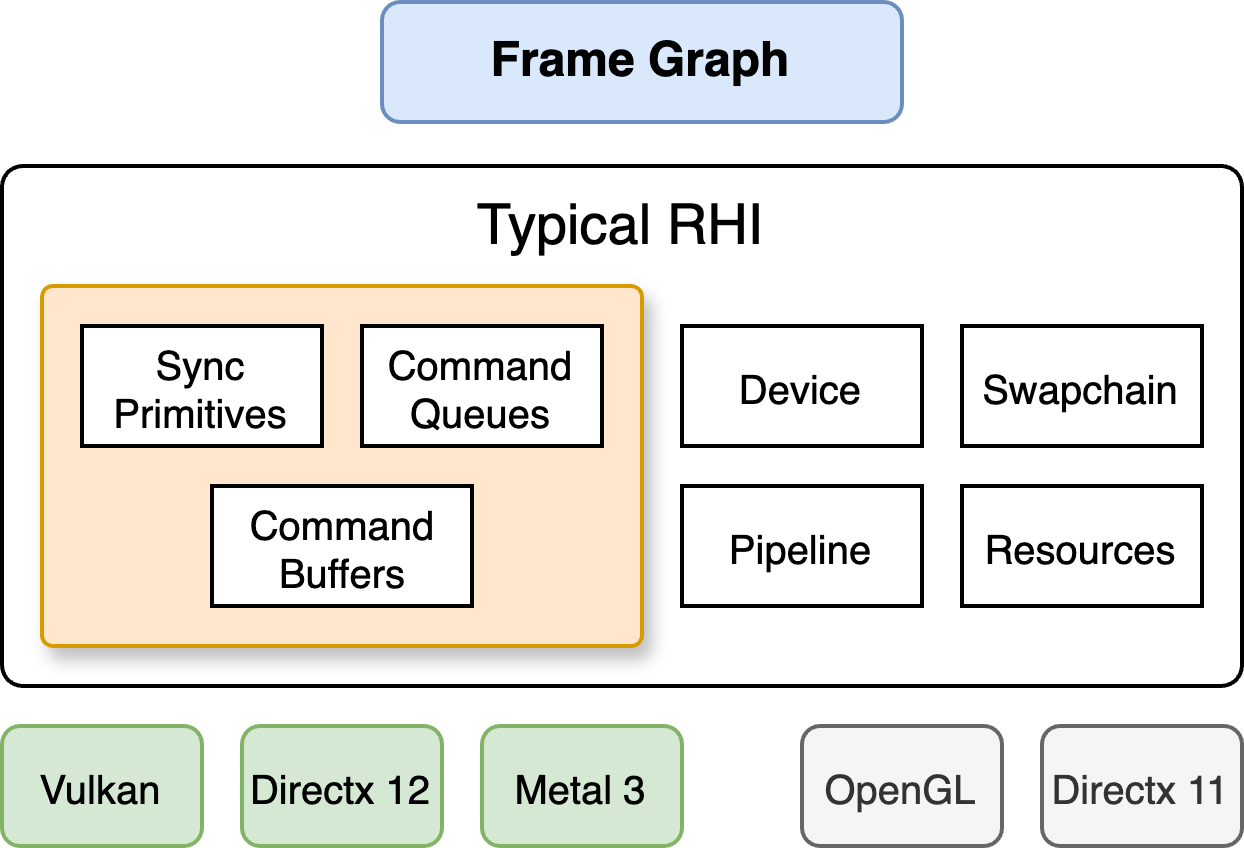
\includegraphics[scale=0.175]{rhi/typical_rhi_diagram.png}
    \hfill
    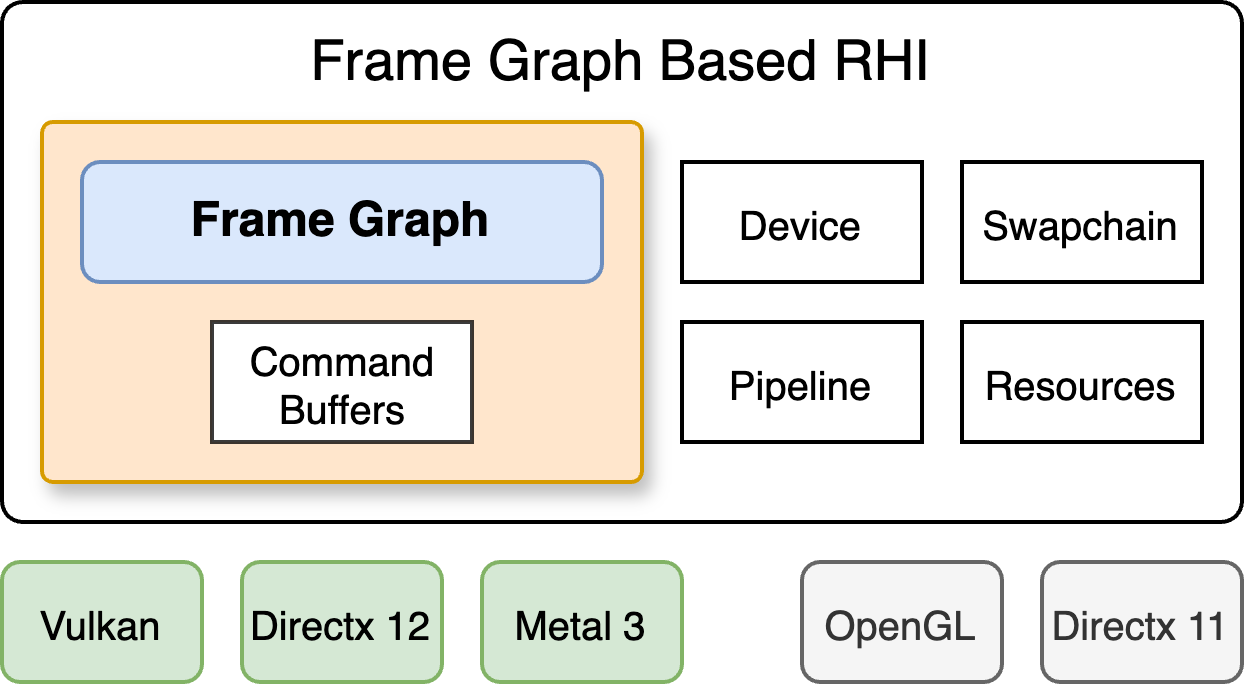
\includegraphics[scale=0.175]{rhi/frame_graph_based_rhi_diagram.png}
    \caption{Сравнение типичного дизайна RHI (слева) и дизайна, предложенного в данной работе, внедряющего кадровый граф напрямую в RHI (справа).}
    \label{fig:rhi_design_comparison}
\end{figure}

На рисунке \ref{fig:rhi_design_comparison} представлено сравнение типичной структуры RHI и структуры, предложенной в данной работе. Как видно из рисунка, получилось избавиться от абстракции примитивов синхронизации и командных очередей. Несмотря на то, что командные буферы остались как класс в RHI, методы их создания и отправки на исполнения не предоставляются -- всем этим занимается кадровый граф. Как уже было сказано, данный подход дает полную свободу при имплементации RHI, поскольку нет необходимости в попытках обобщить интерфейсы всех графических API, как это сделано в типичном дизайне.

\subsubsection{Декларация кадрового графа}
На этапе декларации графа задаются вершины, а также ресурсы, которые будут использоваться. Вершина графа может быть одного из трех типов -- \textit{graphics}, \textit{compute} или же \textit{transfer}. Ресурсы, в свою очередь, могут быть либо вспомогательными, либо импортированными. Первыми владеет и управляет кадрового граф, вторыми же он только пользуется. Каждому использованию ресурса присваивается некоторое уникальное целое число -- \textit{версия}. Пример декларации графической вершины представлен в листинге \ref{lst:render_graph_declaration}. Компиляцией занимается конкретная имплементация RHI, на этом этапе создаются все необходимые объекты для исполнения кадрового графа. На этапе исполнения конкретная имплементация проходит в нужном порядке по вершинам, вызывает задачу, ассоциированную с данной вершиной на этапе декларации и занимается автоматически расстановкой синхронизации, контекста, отправляет работу на графический процессор и т.д.

\begin{minipage}[h]{0.95\textwidth}
\centering
\begin{cpp}[language=C++, caption={Пример декларации графической вершины графа.}, label={lst:render_graph_declaration}]
auto rg_color = builder.DeclareImportTexture(...);
auto rg_depth = builder.DeclareTransientTexture(...);

builder.BeginRenderPass("Forward Pass");
builder.AddColorTarget(rg_color, ...);
builder.SetDepthStencil(rg_depth, ...);
builder.SetJob([](CommandBuffer& cmds) {
    ...
});
builder.EndRenderPass();
\end{cpp}
\end{minipage}

Часто бывает необходимо декларировать временные ресурсы, чьи параметры зависят от других ресурсов. Например, это может быть буфер глубины, ведь его размер должен совпадать с размерами окна, т.е. главного рендер таргета. В связи с этим функции декларации временных ресурсов принимают структуру, похожую на обычную спецификацию ресурса, но у которой некоторые поля (такие как напр. размер) могут помимо точного значения принимать версию ресурса кадрового графа, показывая зависимость. Пример такой декларации показан в \ref{lst:render_graph_dependent_texture_info}.

\begin{minipage}[h]{0.95\textwidth}
\centering
\begin{cpp}[language=C++, caption={Пример декларации зависимых временных ресурсов.}, label={lst:render_graph_dependent_texture_info}]
auto rg_color = builder.DeclareImportTexture(...);

rhi::FrameGraph::DependentTextureInfo depth_info{};
depth_info.extent.SetDependency(rg_color);
depth_info.format = rhi::Format::D32_SFLOAT;
depth_info.type   = rhi::TextureType::Texture2D;
depth_info.usage  = rhi::DeviceResourceState::DepthStencilTarget;
...
depth_info.name   = "Depth buffer";

auto rg_depth = builder.DeclareTransientTexture(depth_info);
\end{cpp}
\end{minipage}

\subsection{Алгоритм компиляции}
\subsubsection{Топологическая сортировка}
\begin{wrapfigure}{R}{0.305\textwidth}
    \centering
    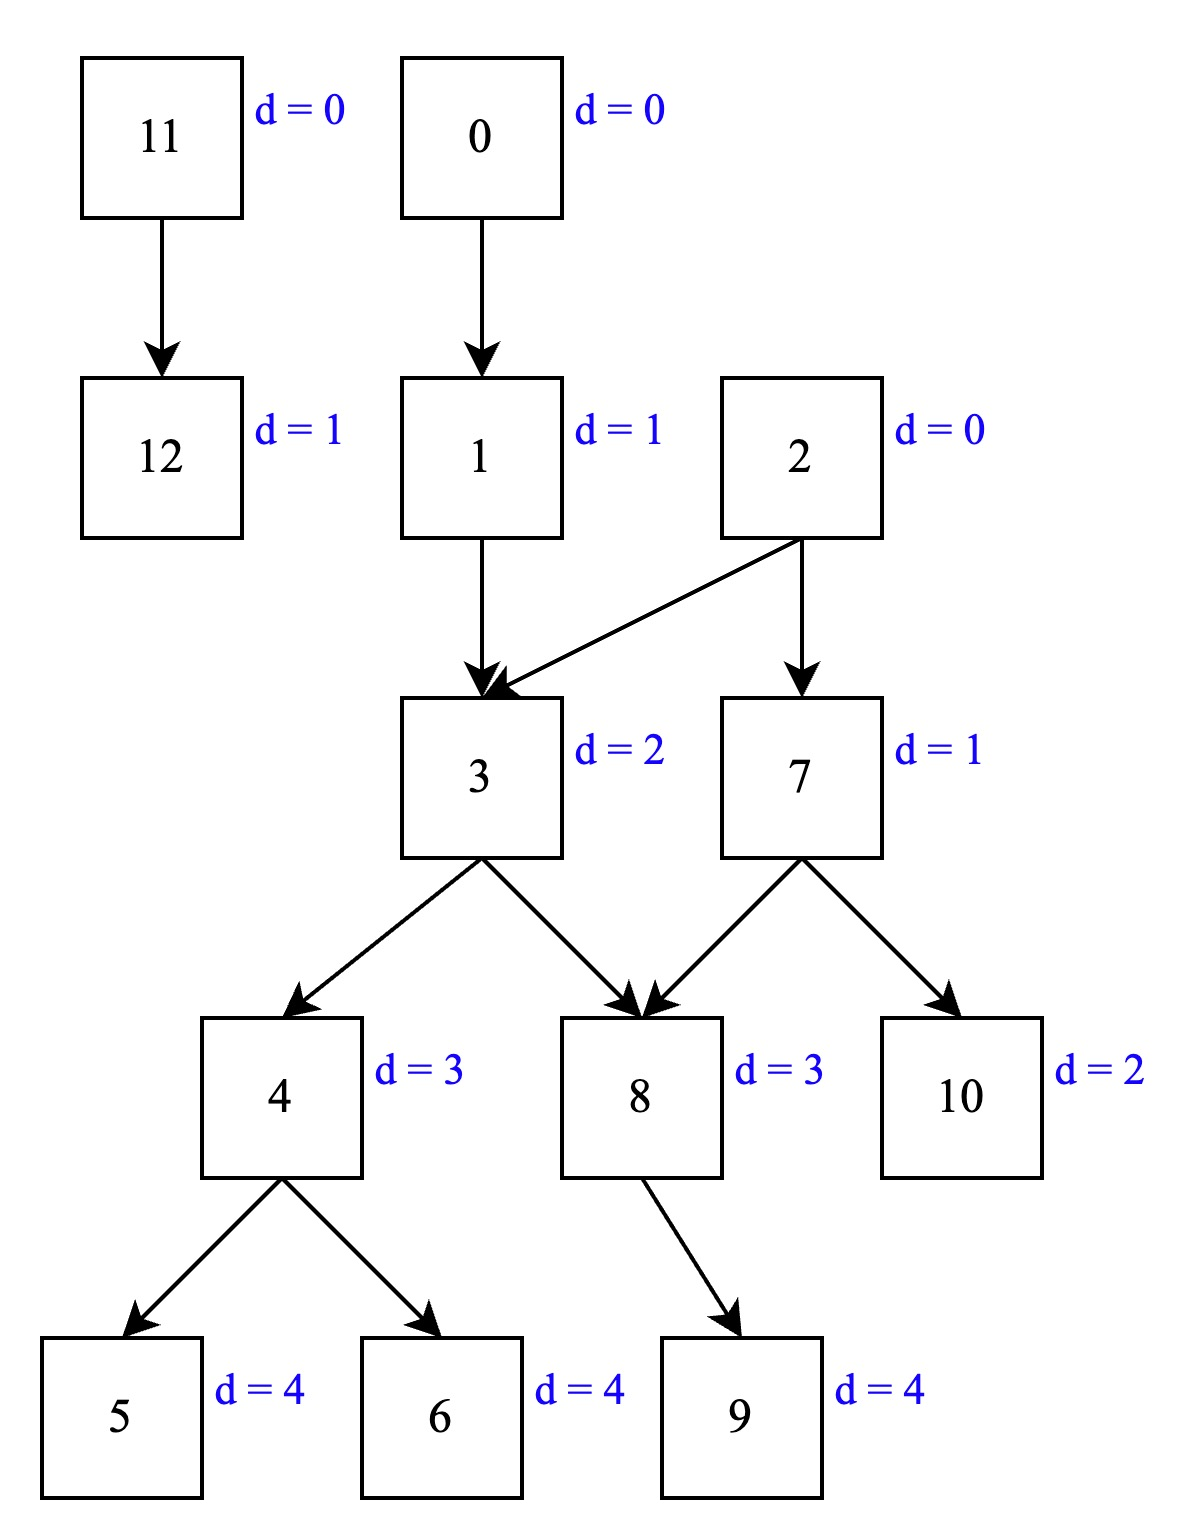
\includegraphics[scale=0.115]{rhi/render_graph/topological_sort_graph.jpeg}
    \caption{Граф зависимостей.}
    \label{fig:render_graph_topological_sort_graph}
\end{wrapfigure}

Первая часть компиляции кадрового графа -- топологическая сортировка, она является универсальной для всех имплементаций. Предположим у нас есть $V$ вершин графа и уже расставленные ребра между ними, где ребро $(u, v)$, означает что вершина $v$ должна исполняться после $u$. В дальнейшем нам также понадобится глубина (или по-другому \textit{dependency level}) каждой вершины, обозначим ее $d(u)$. Глубина вершины помогает определить какие вершины потенциально могут исполняться параллельно. Она определяется как минимальная из всех возможных реберная длина пути от некоторой вершины $s$, в которую не ведут никакие ребра. За один обход в глубину графа мы сможем получить как глубины всех вершин, так и некоторую топологическую сортировку. Однако произвольная топологическая сортировка нам не подойдет. Необходимо, чтобы в получившейся сортировке глубины вершин монотонно не убывали. Для этого необходима дополнительная сортировка массива. Результат данной части алгоритма для графа \ref{fig:render_graph_topological_sort_graph} проиллюстрирован на рисунке \ref{fig:render_graph_topological_sort_arrays}. Данная часть алгоритма позволяет преждевременно обнаружить циклические зависимости и обеспечивает корректный порядок всех задач в графе. Кроме того, монотонное неубывание глубин помогает в дальнейшем распределении ресурсов и синхронизации выполнения.

\begin{figure}[h]
    \centering
    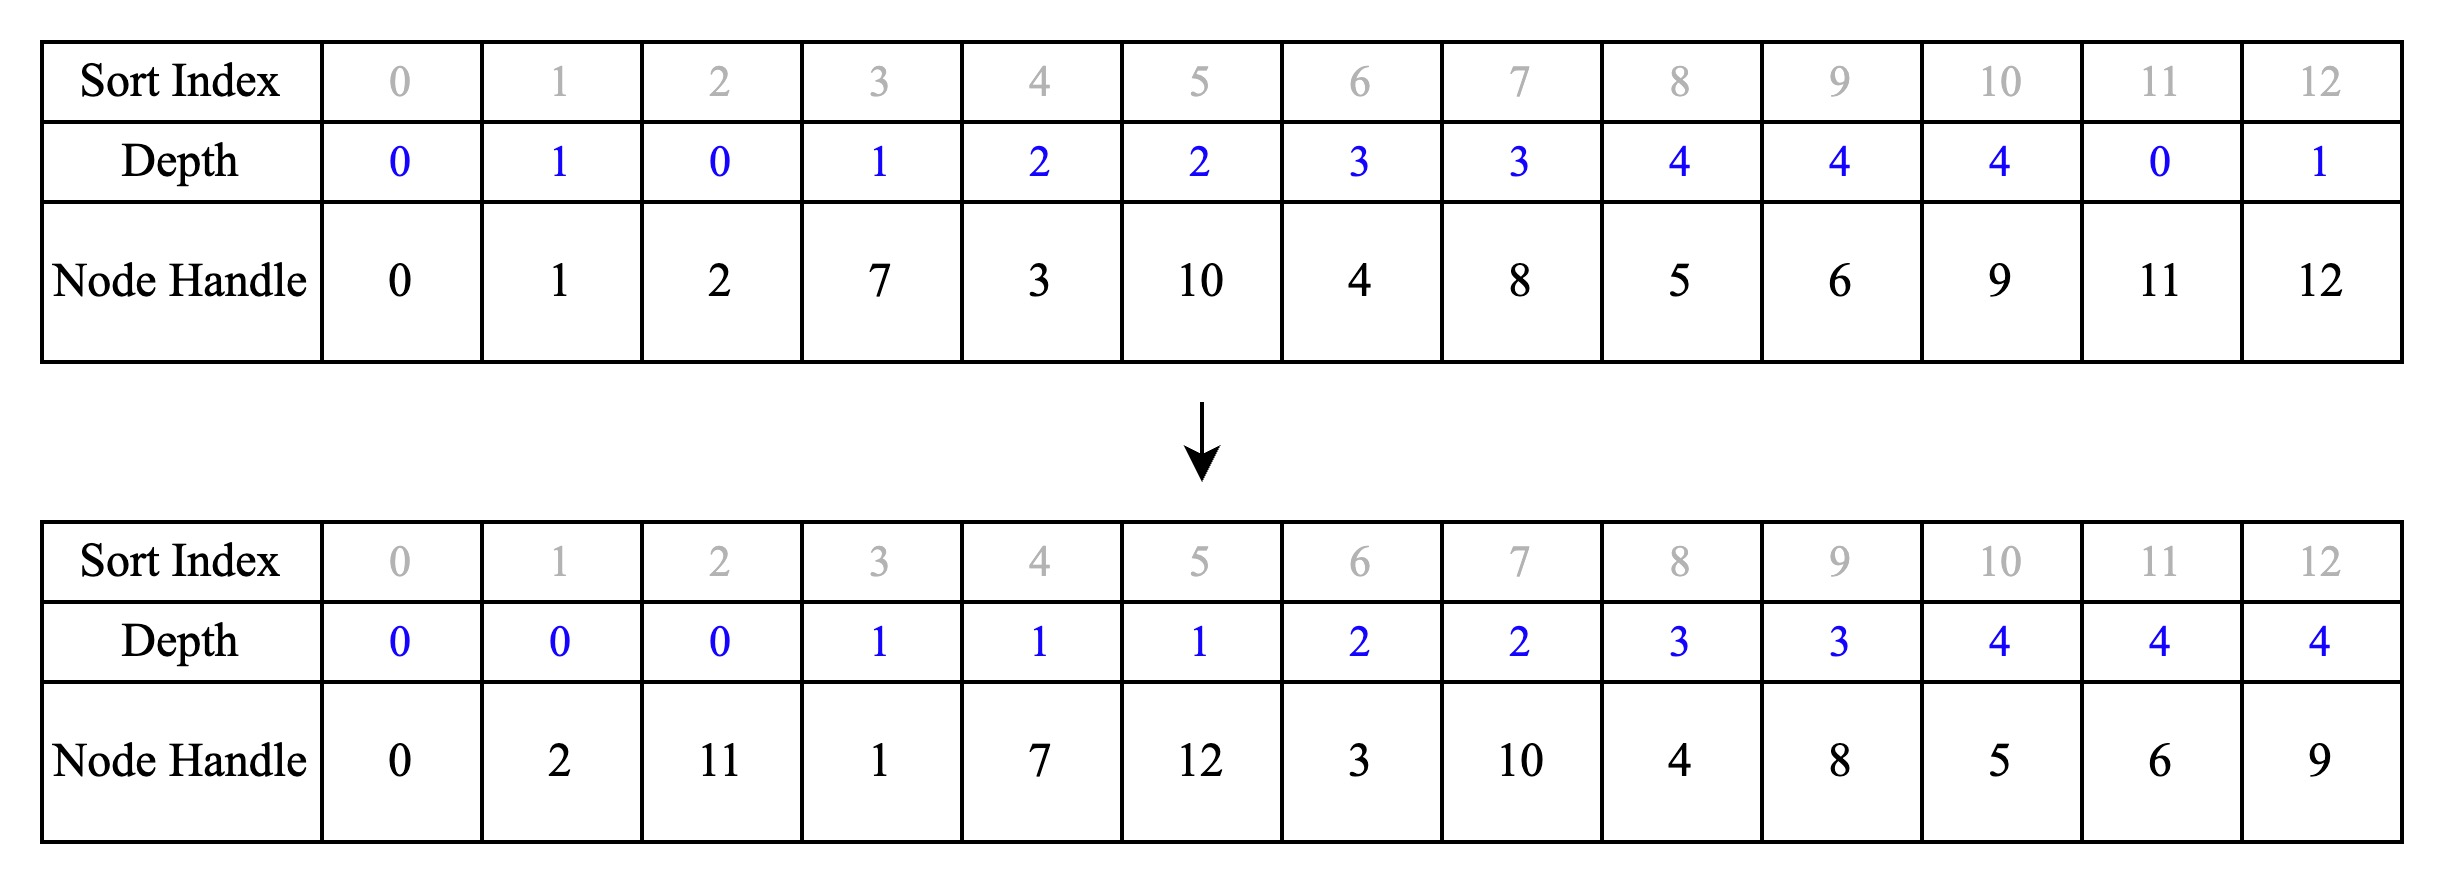
\includegraphics[scale=0.15]{rhi/render_graph/topological_sort_array.jpeg}
    \caption{Первый массив -- произвольная топологическая сортировка, второй -- перестановка первого, упорядочивающая глубину по неубыванию (оставаясь при этом топологической сортировкой).}
    \label{fig:render_graph_topological_sort_arrays}
\end{figure}

\subsubsection{Отсечение ребер}
Теперь избавимся от ненужных ребер графа для дальнейшего определения точек синхронизации командных очередей. Этот этап критически важен для оптимизации работы графа и уменьшения накладных расходов на синхронизацию. Данная часть алгоритма основана на статье \cite{organizing_gpu_work_with_directed_acyclic_graphs} и идентична для всех современных графических API. Предположим, у нас есть $Q$ командных очередей. Также для каждой вершины нам известен индекс очереди, на которой она будет исполняться -- $queue\_idx(u) \in \{0,...,Q-1\}$. Прежде всего необходимо переиндексировать вершины так, чтобы внутри каждой очереди вершины шли по возрастанию, и для любой пары очередей $q_1, q_2 \in \{0,...,Q-1\}$, таких что $q_1 < q_2$, все вершины очереди $q_1$ имели индексы меньше, чем индексы всех вершин очереди $q_2$. Положим в качестве такой переиндекцации $\sigma(u) = sort\_idx(u) + queue\_idx(u) \cdot V + 1$. Также для каждой вершины введем так называемый \textit{Sufficient Synchronization Index Set} (сокращенно \textit{SSIS}), для каждой очереди показывающий индекс $\sigma$ вершины, с которой достаточно синхронизировать данную вершину. Формальное определение \textit{SSIS} представлено в равенстве \ref{eq:ssis_definition}. Граф с посчитанными \textit{SSIS} можно увидеть на рисунке \ref{fig:cross_queue_graph_original}.

\begin{align}
    i_{q}(u) &= \left\{ \begin{array}{rcl}
        \sigma(u) & \mbox{если} & q = queue\_idx(u) \\
        0 & \mbox{иначе, если} & \forall v: (u, v) \notin E(G^R) \\
        \underset{d(v) \leq d(u)}{\underset{(u,v) \in E(G^R)}{\arg\max}} \{\sigma(v)\} & \mbox{иначе}
    \end{array}\right.&\\
    SSIS(u) &= \left( i_0(u), ..., i_{Q-1}(u) \right) \label{eq:ssis_definition}
\end{align}

Строить новый граф без лишних ребер (назовем его $G^*$) будем итеративно. Для начала для каждой вершины посчитаем бинарный кортеж $cover$ из $Q$ элементов, каждый элемент которого показывает синхронизирована ли уже данная вершина с данной очередью. Дальше будем в цикле пытаться улучшить ситуацию, пока для всех вершин $cover$ не станет полностью из единиц. На каждой итерации раскрываются все вершины $u$, чьи $cover$ имеют нули. Раскрытие вершины $u$ происходит следующим образом: рассматриваются все вершины $v$, в которые идут ребра реверс графа из $u$, считается промежуточный $cover$ между только этими двумя вершинами, и если данное ребро улучшает глобальный $final\_cover(u)$, то мы запоминаем вершину $v$. Выбрав из всех таких $v$ наилучшую (по количеству единиц, которое она добавляет в $final\_cover(u)$), мы обновляем $final\_cover(u)$ и добавляем в граф $G^*$ ребро $(u, v)$. Полный алгоритм представлен в листинге \ref{lst:render_graph_cross_queue_graph}, а также первая итерация алгоритма проиллюстрирована на рисунке \ref{fig:cross_queue_graph_first_iteration}.
\begin{figure}[htp]
    \begin{subfigure}
        \centering
        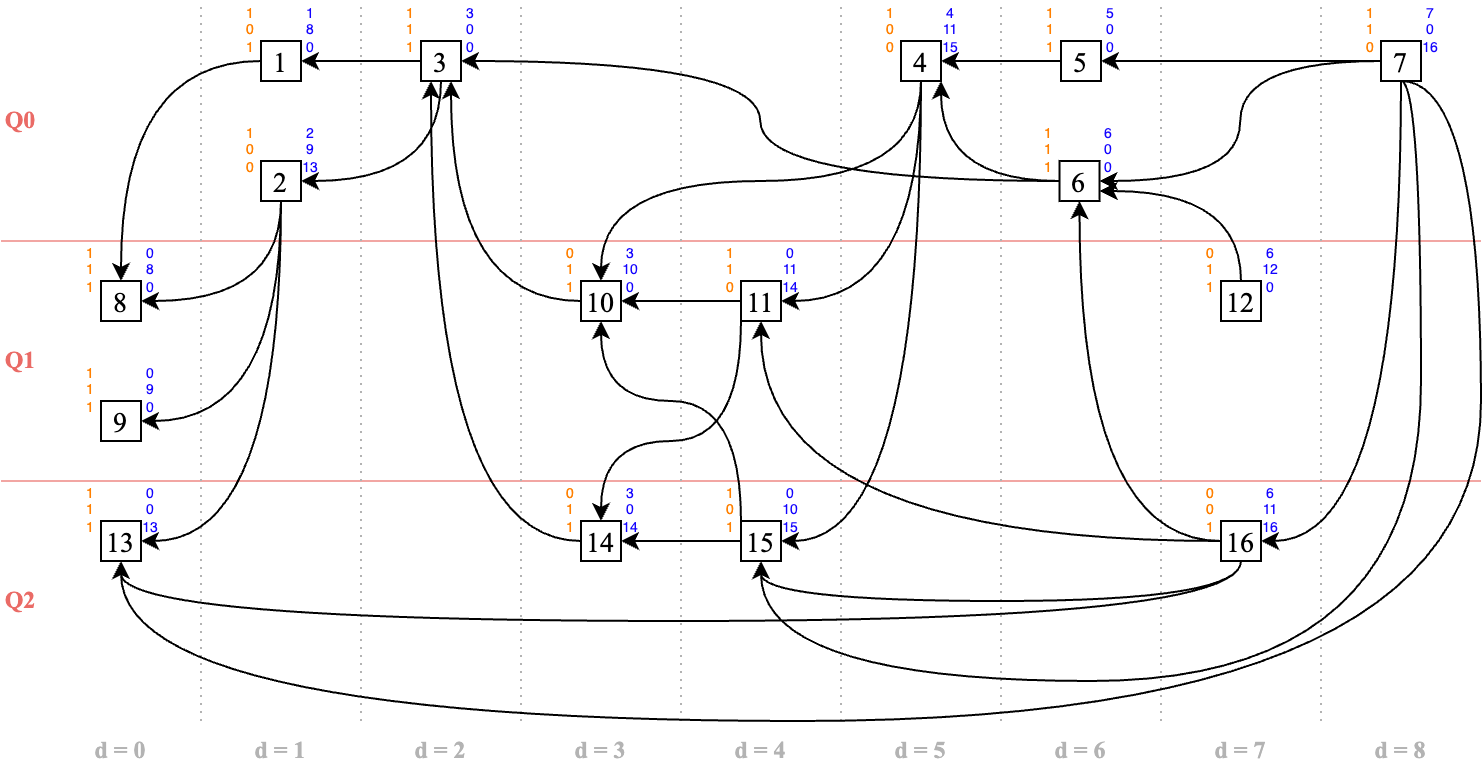
\includegraphics[scale=0.315]{rhi/render_graph/cross_queue_graph_original.png}
        \caption{Изначальный реверс граф, где у каждой вершины справа синим светом подписан $SSIS$, слева оранжевым $final\_cover$, а индексация вершин показывает $\sigma(u)$.}
        \label{fig:cross_queue_graph_original}
    \end{subfigure}
    \bigskip
    \bigskip
    \begin{subfigure}
        \centering
        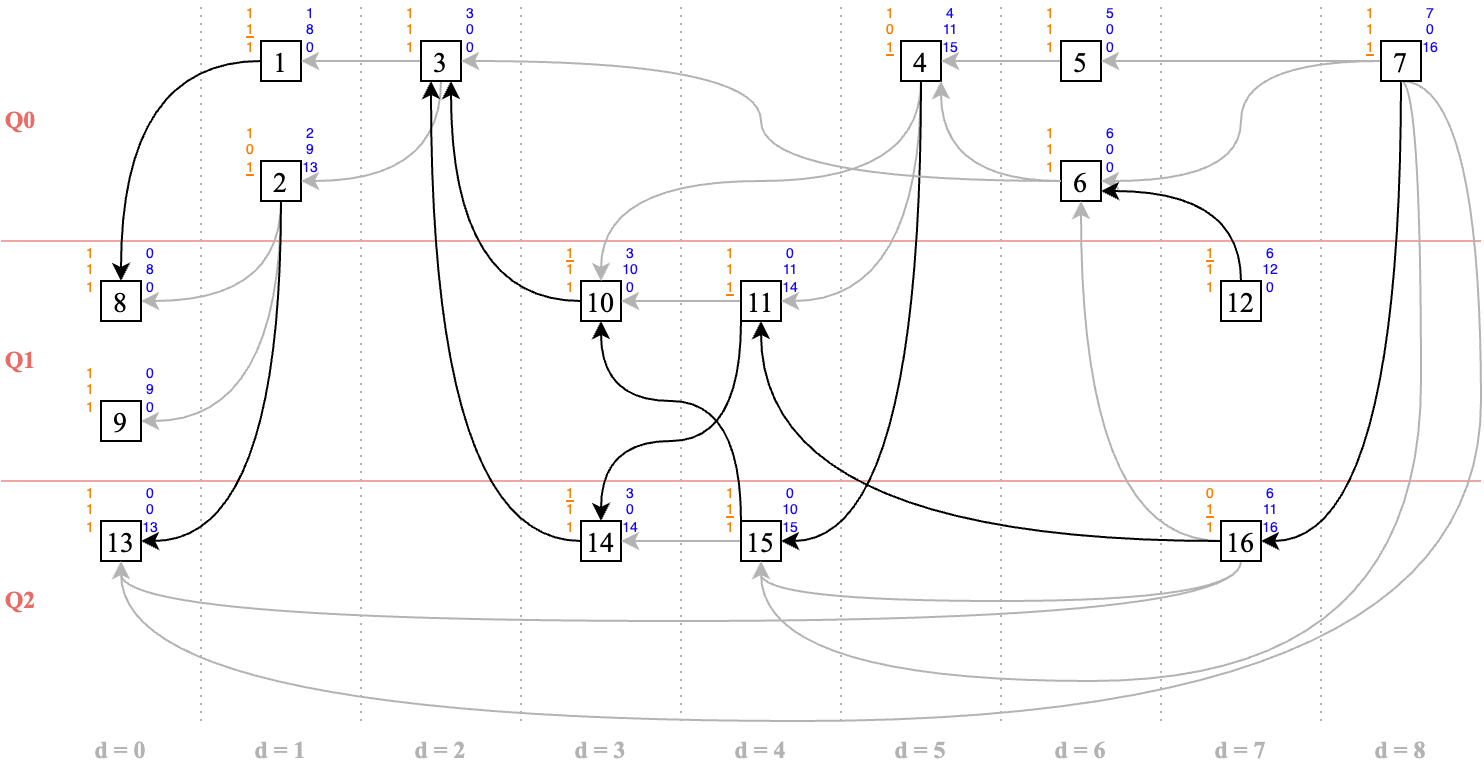
\includegraphics[scale=0.315]{rhi/render_graph/cross_queue_graph_first_iteration.png}
        \caption{Первая итерация алгоритма построения $G^*$.}
        \label{fig:cross_queue_graph_first_iteration}
    \end{subfigure}
\end{figure}

\begin{minipage}[t]{0.95\textwidth}
    \centering
    \begin{pseudocode}[mathescape=true, caption={Построение графа $G^*$ с достаточным минимальным набором ребер для межочередной синхронизации}, label={lst:render_graph_cross_queue_graph}]

    function CoverScore($cover$):
        return $\sum_{q=0}^{Q-1} cover_q$

    $\forall u: final\_cover(u) \leftarrow (1, ..., 1)$
    $\forall u \forall q \in\{0, ..., Q-1\}: (\exists v: (u, v) \in E(G^R)) \implies final\_cover_q(u) \leftarrow 0$

    $covered\_all$ $\leftarrow$ false
    while not $covered\_all$:
        $covered\_all$ $\leftarrow$ true
        for $u \in G^R$:
            $v^* \leftarrow \emptyset$
            $cover^* \leftarrow final\_cover(u)$
            for $v \in G^R, (u, v) \in E(G^R)$:
                $cover \leftarrow (..., SSIS_q(u) \leq SSIS_q(v), ...)$
                if CoverScore($cover$) $>$ CoverScore($cover^*$):
                    $v^* \leftarrow v$
                    $cover^* \leftarrow cover$
                else if CoverScore($cover$) $=$ CoverScore($cover^*$) and $\sigma(v) > \sigma(v^*)$
                    $v^* \leftarrow v$
                    $cover^* \leftarrow cover$
            if $v^* \neq \emptyset$:
                $final\_cover(u) \leftarrow final\_cover(u) | cover^*$
                $G^* \leftarrow G^* \cup (u, v^*)$
            if CoverScore($final\_cover(u)$) $\neq Q$:
                $covered\_all$ $\leftarrow$ false
    \end{pseudocode}
\end{minipage}

\subsubsection{Синхронизация}
Дальше идет часть компиляции, во многом уникальная для Vulkan. Нам необходимо расставить сабмиты, а также синхронизацию между ними при помощи семафоров (примитивов синхронизации командных очередей). В новых версиях Vulkan появились так называемые \textit{timeline semaphores} (временные семафоры) \cite{vulkan_timeline_semaphore}, способные хранить 64-битное число вместо бинарного флага. Поэтому в данной работе предлагается использовать именно их, ввиду их гибкости и сильного снижения количества необходимых примитивов синхронизации.

Сабмиты ставятся в конце каждой командной очереди, а также после каждого уровня глубины, на котором существует хотя бы одна вершина, в которую есть входящие ребра графа $G^*$. Такой подход гарантирует необходимую синхронизацию и при этом не влечет излишних задержек. На каждую командную очередь выделяется по одному временному семафору. Поскольку значения должны монотонно возрастать, каждое значение можно представить как $$Timepoint(frame\_idx, submit\_idx) = frame\_idx \cdot V + submit\_idx \text{.}$$
В данном определении $V$ -- произвольное число, заведомо большее числа сабмитов на каждой очереди, а $submit\_idx$ -- индекс сабмита на конкретной очереди в 1-индексации. Дальше достаточно на основе ребер $G^*$ расставить значения ожидания/сигнала на каждом сабмите. Финальную версию графа $G^*$ с выставленными сабмитами можно увидеть на диаграмме \ref{fig:cross_queue_graph_submits}.

Немаловажной частью работы с Vulkan также является ручная расстановка барьеров исполнения для ресурсов. Правильная расстановка барьеров критична для предотвращения ошибок гонки данных. Если ресурс используется исключительно в одной очереди, то автоматическая расстановка барьеров в таком случае тривиальна, хотя и требует внимательного рассмотрения всех параметров. Сложность возникает, когда ресурс используется на нескольких очередях. Самый простой вариант решения данной проблемы -- это создание всех ресурсов с указанием автоматического кросс-очередного использования. Однако этот подход может повлиять на производительность, например, делая невозможным использование \textit{delta color compression} \cite{optimising_a_aaa_vulkan_title_on_desktop}. Второй же подход -- расставлять барьеры с \textit{queue ownership transfer}. В целом, в текущей имплементации графа расстановка данных барьеров не требует больших усилий, поэтому этот подход более предпочтительный.

\begin{figure}[h]
    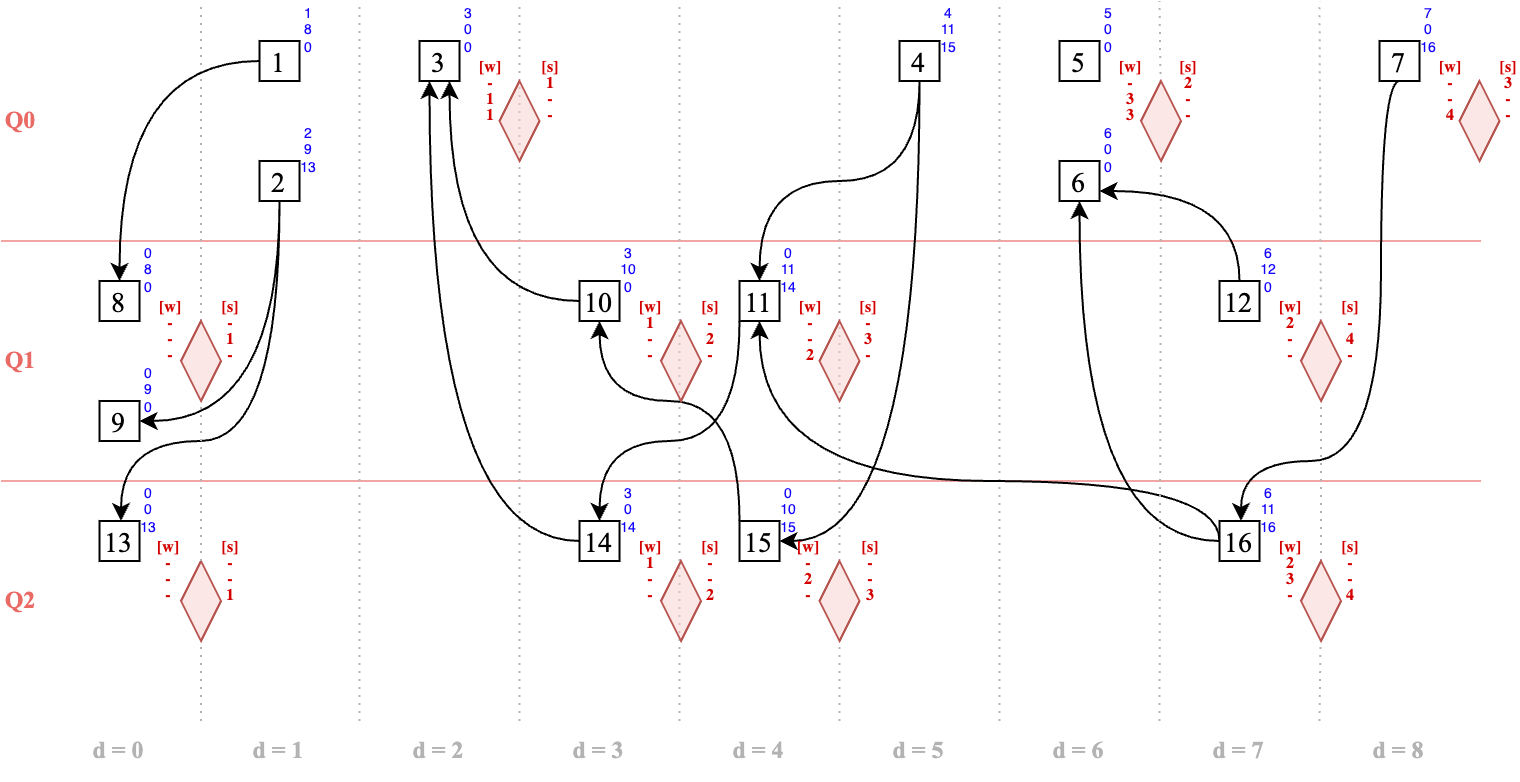
\includegraphics[scale=0.308]{rhi/render_graph/cross_queue_graph_submits.png}
    \caption{Финальный граф $G^*$ с выставленными сабмитами. Слева от каждого сабмита подписаны значения для ожидания на каждую очередь, а справа -- значения для сигнала.}
    \label{fig:cross_queue_graph_submits}
\end{figure}

\subsection{Отладочная информация}
Для отладки были разработаны два вида визуализации конкретных кадровых графов с помощью инструмента Graphviz \cite{graphviz} -- краткая и подробная. Краткая версия предоставляет общую картину графа, что помогает быстро определить корректность "потока" ресурсов в графе. Подробная же отображает дополнительно все параметры ресурсов, типы их использования, а также барьеры. Эта информация особенно полезна при выявлении узких мест и оптимизации производительности рендеринга. Дополнительно, проставляются имена ресурсов и вершин, а также именные границы команд в командных буферах по тому, какой вершине они принадлежат, с помощью специального расширения для Vulkan -- VK\_EXT\_debug\_utils \cite{vulkan_ext_debug_utils}. Данная информация помогает при графической отладке в приложениях, таких как RenderDoc \cite{renderdoc}. Пример показан на рисунке \ref{fig:renderdoc_capture_debug_utils}. Представленные механизмы позволяют легко идентифицировать причины ошибок и конфликтующие зависимости между ресурсами, что значительно ускоряет процесс разработки.

\begin{figure}[h]
    \centering
    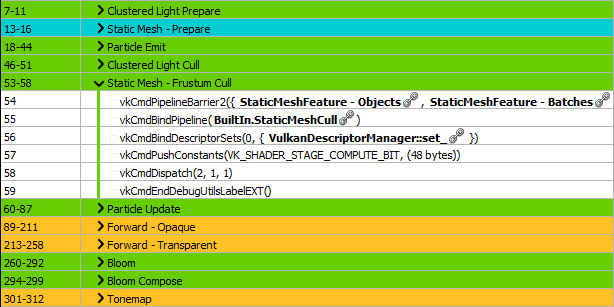
\includegraphics[scale=0.7]{rhi/renderdoc_capture_debug_utils.jpg}
    \caption{Скриншот из RenderDoc, показывающий этапы встроенного рендерера (синий цвет означает transfer, зеленый означает compute и оранжевый -- graphics), а также отображающий имена ресурсов (см. события 54-56).}
    \label{fig:renderdoc_capture_debug_utils}
\end{figure}

\subsection{Структура кадра}
В отличие от оригинального решения, предложенного в \cite{frame_graph_frostbite}, в данной работе была реализована возможность наличия нескольких кадровых графов. Существует два способа исполнения графов -- последовательное и асинхронное. Последовательное исполнение синхронизируется при помощи временных семафоров, аналогично механизму синхронизации сабмитов, разобранному в пункте про компиляцию графов. В данном случае формула момента времени становится $$Timepoint(frame\_idx, graph\_idx) = frame\_idx \cdot G + graph\_idx\text{,}$$где $G$ -- произвольное число, заведомо большее числа графов на кадр. При асинхронном же исполнении синхронизации не происходит. Завершение асинхронного исполнения можно проверить вручную, либо же указав callback при отправке графа на исполнение. Возможность наличия нескольких кадровых графов позволяет более гранулярно разбить разные модули игрового движка, занимающиеся работой с GPU. Так, например, на рисунке \ref{fig:several_render_graphs} представлено возможное разбиение работы на: рендеринг игры, рендеринг в инструментах редактора, отрисовка пользовательского интерфейса, а также асинхронный трансфер данных и генерация preview изображений для редактора. Такой подход позволяет легко масштабировать систему, добавляя новые графы для концептуально новых задач без изменений в уже существующих. Использование нескольких кадровых графов также обеспечивает изоляцию между различными подсистемами, что повышает стабильность и упрощает отладку.

\begin{figure}[h]
    \centering
    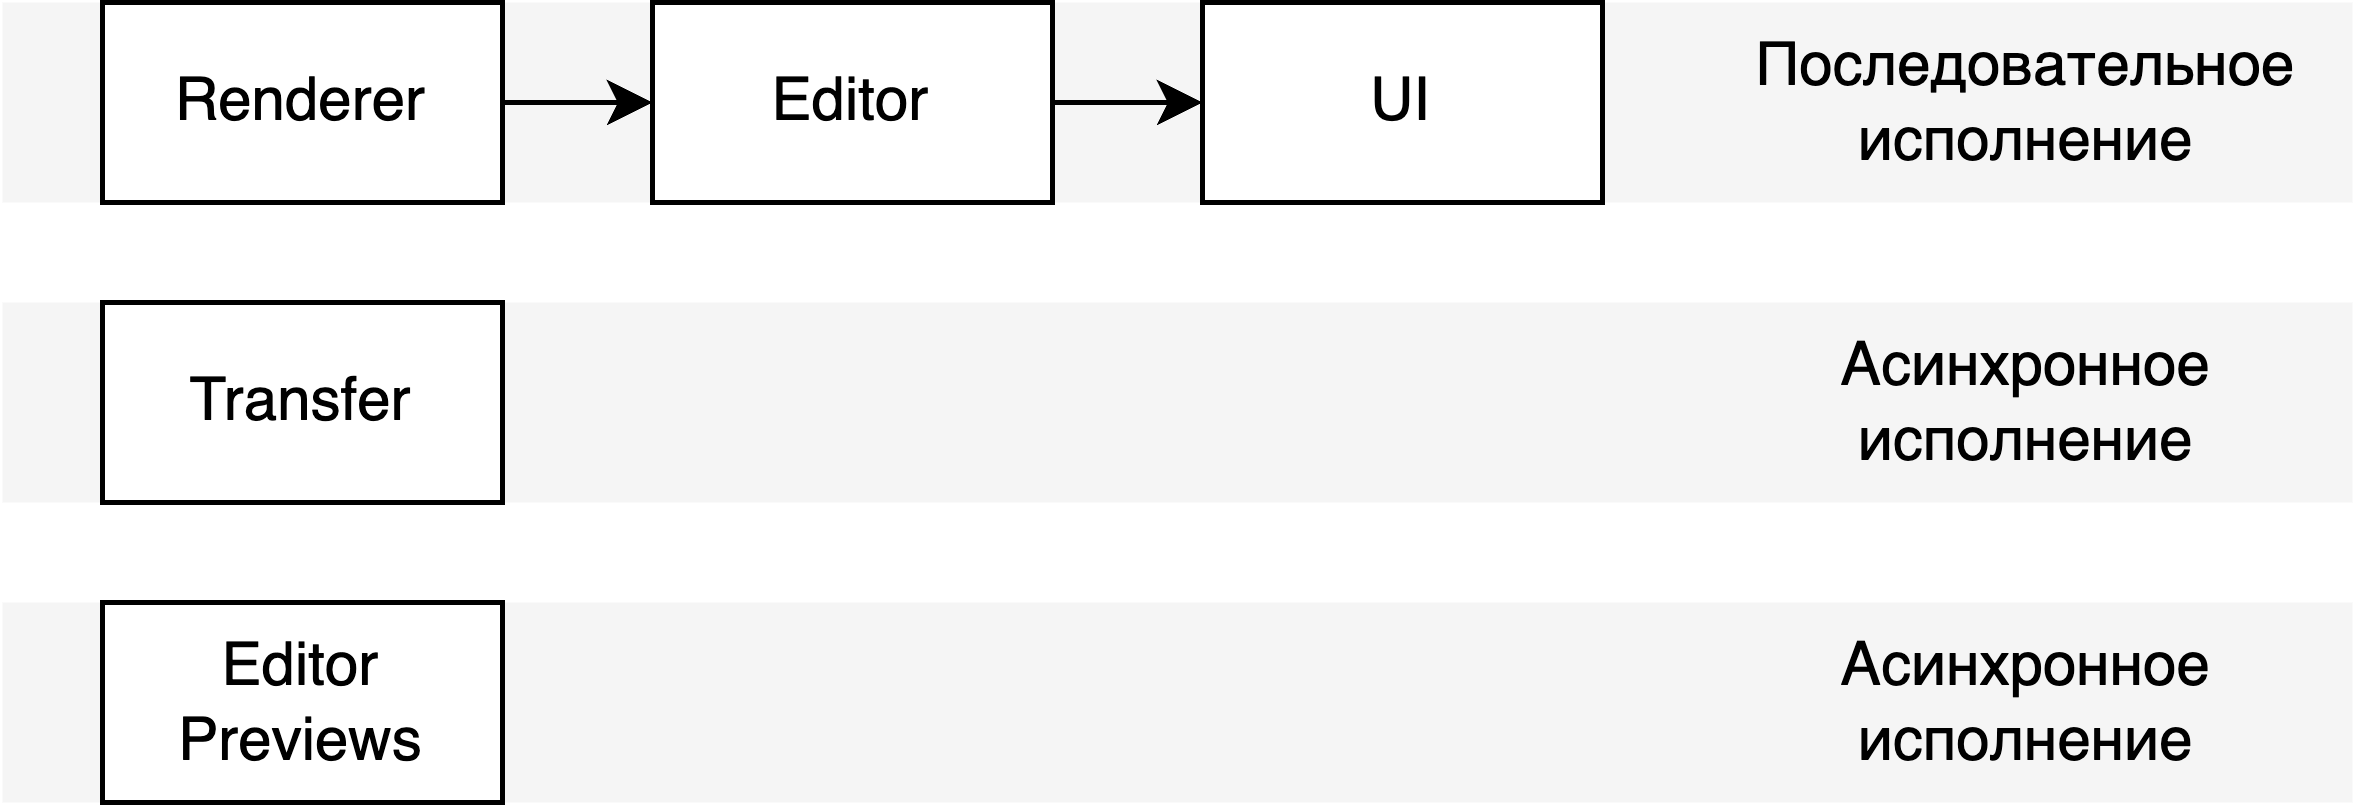
\includegraphics[scale=0.15]{rhi/render_graph/several_render_graphs.png}
    \caption{Виды композиции исполнения кадровых графов и примеры использования данной функции.}
    \label{fig:several_render_graphs}
\end{figure}
\newpage
\section{Применение в высокоуровневом рендеринге}
В данной главе представлена имплементация высокоуровнего рендерера в целях тестирования дизайна и реализации RHI. Современный высокоуровневый рендерер должен быть модульным, удобным в использовании, а также в идеальном случае быть полностью конфигурируемым, включая возможность написания кастомного решения специально под нужды конкретного игрового проекта.

\subsection{Общий дизайн}
Дизайн, представленный в данной работе (см. рисунок \ref{fig:renderer_design}) стремится решить все эти проблемы. Рендерер состоит из абстрактных компонент -- IRenderFeature. Каждая из них декларирует вершины рендер графа, а также ECS системы (в основном предназначенные для агрегирования данных из компонент сущностей на сцене). Коммуникация между различными IRenderFeature сделана через абстрактный Context, способный содержать произвольные данные.

\begin{figure}[h]
    \centering
    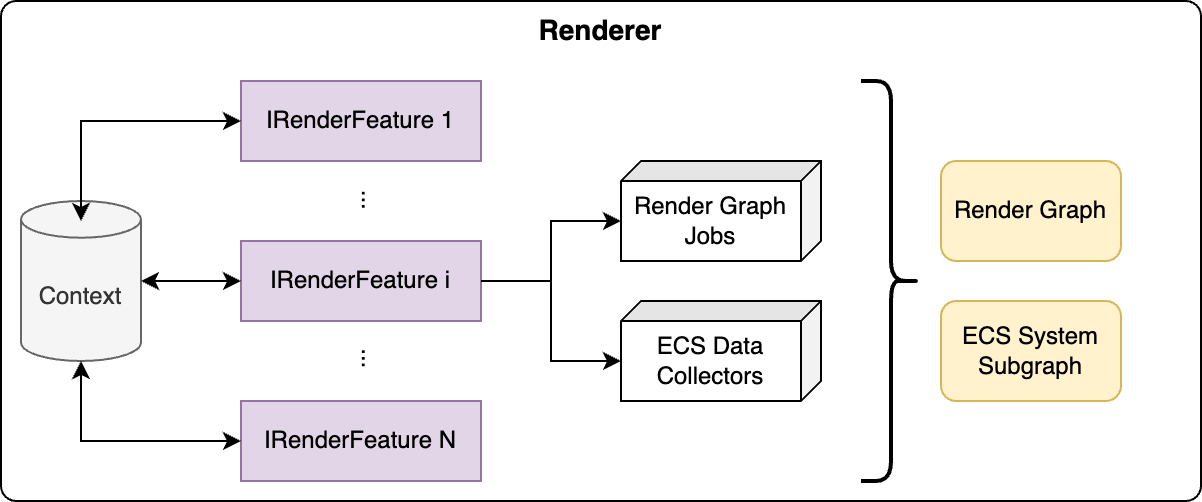
\includegraphics[scale=0.33]{renderer/renderer.png}
    \caption{Дизайн рендерера}
    \label{fig:renderer_design}
\end{figure}

Конкретные имплементации IRenderFeature можно классифицировать на: отрисовку геометрии, отрисовку процедурных объектов, а также эффекты постобработки. Поэтому в качестве рендерера по-умолчанию были реализованы методы рендеринга из всех данных классов в качестве проверки дизайна. Список реализованных IRenderFeature и вершины графа каждой из них представлены схематично на \ref{fig:built_in_renderer}.

\begin{figure}[h]
    \centering
    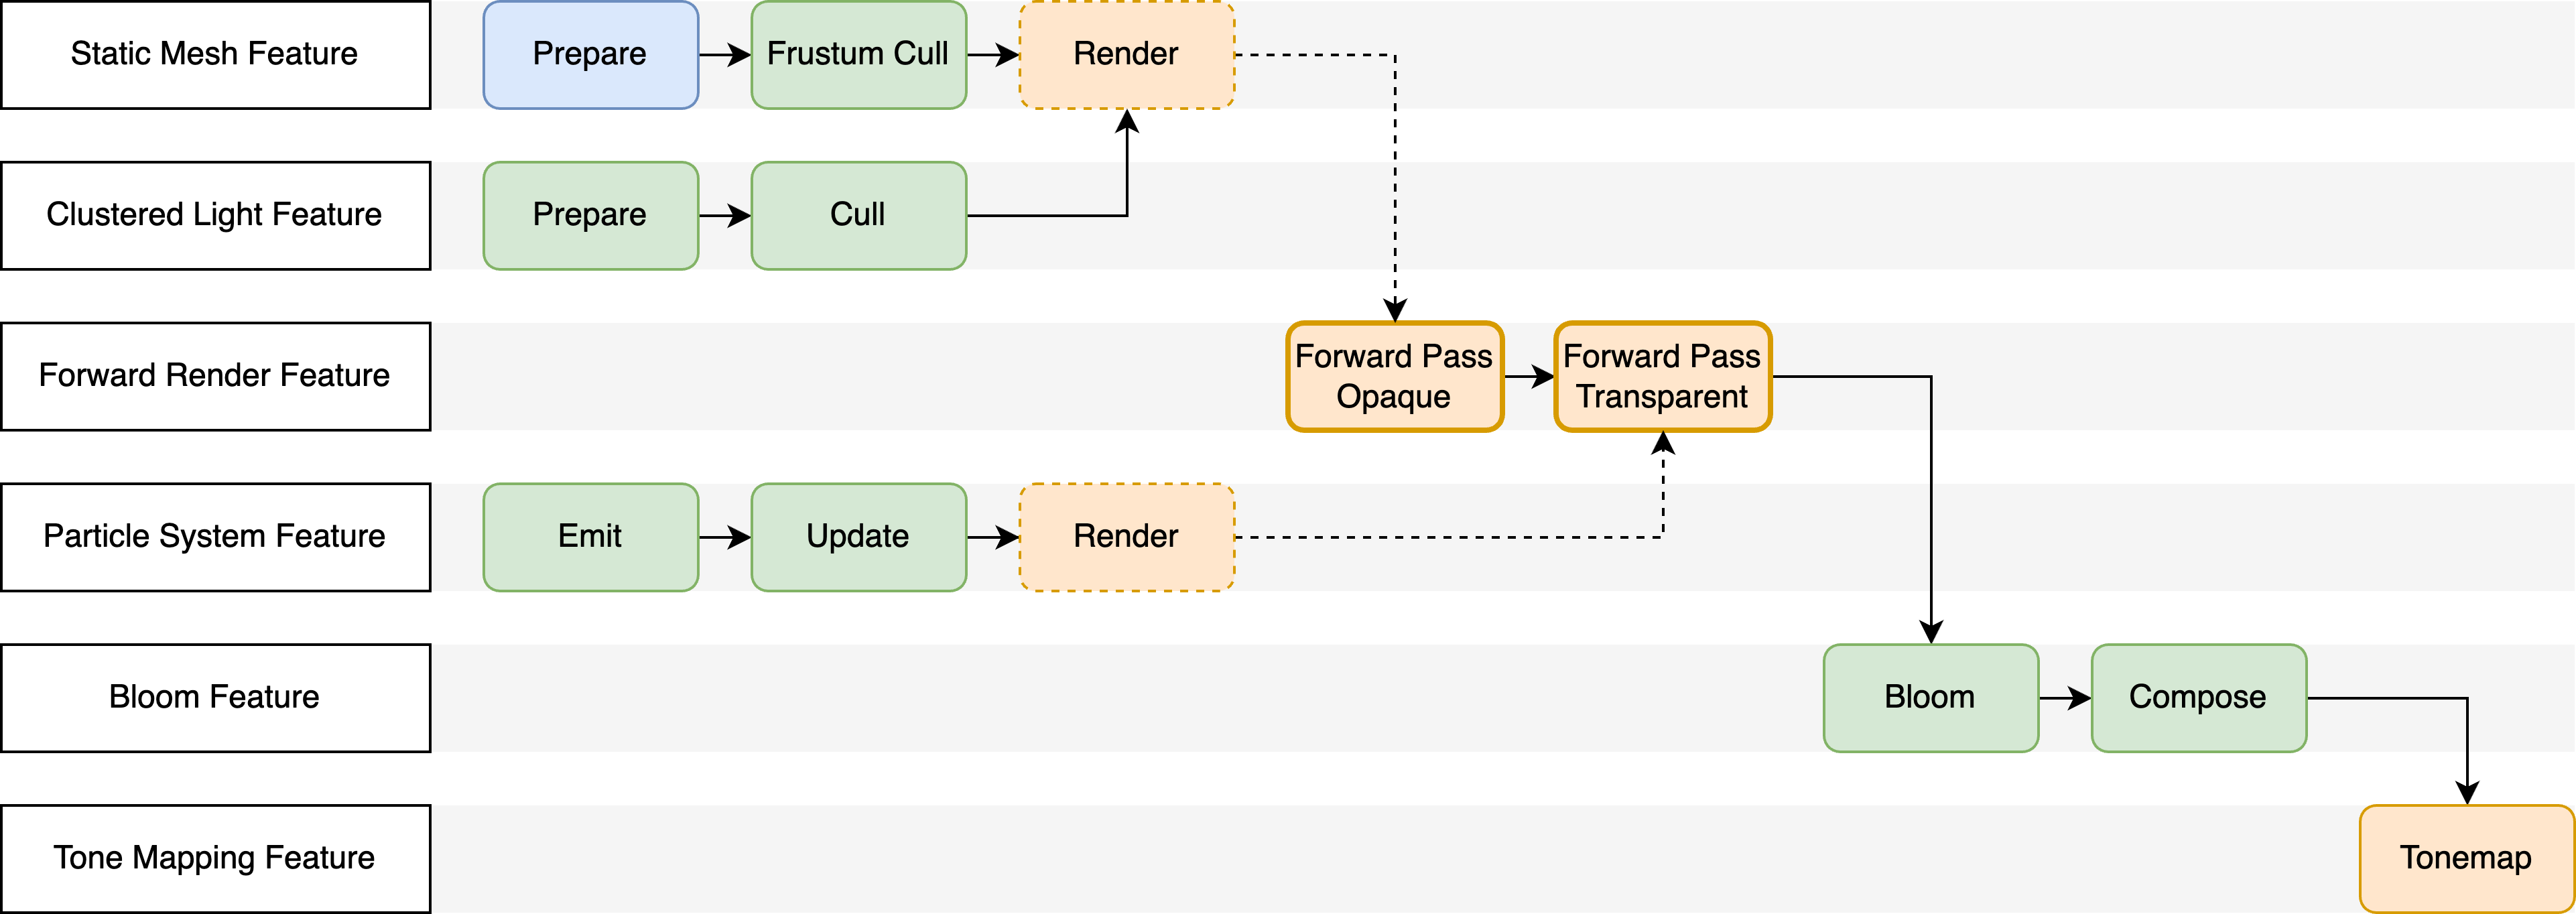
\includegraphics[scale=0.121]{renderer/built_in_renderer.png}
    \caption{Схема имплементации рендерера, представленной в данной работе далее.}
    \label{fig:built_in_renderer}
\end{figure}

\subsection{Отрисовка геометрии}
Еще до появления современных графических API, было стремление к так называемому GPU-Driven Rendering \cite{ubisoft_gpu_driven_rendering} (рендерингу, управляемому GPU), который представляет собой ряд решений, возлагающих значительную работу по генерации команд отрисовки напрямую на GPU. C увеличением комплексности сцен в видеоиграх, возникла необходимость в перераспределении задач таким образом, чтобы максимально использовать возможности GPU. Этот подход использует возможности параллельной обработки современных графических процессоров для выполнения таких задач, как отсеивание, сортировка и генерация вызовов отрисовки. Рендеринг геометрии -- основная цель данного метода. Поэтому было принято решение его задействовать.

У представленного метода два этапа -- отсечение по пирамиде видимости и растеризация видимой геометрии. Первый этап происходит в вычислительном шейдере, и помимо непосредственной проверки видимости каждого объекта он также генерирует косвенный буфер комманд на GPU. Предположим, есть $N$ мешей, каждый из которых используется на сцене потенциально несколько раз. Соберем все экземпляры каждого меша в $N$ групп. Каждая группа будет одним непрямым вызовом отрисовки экземпляров. В командный буфер запишется лишь одна команда -- multi draw instanced indirect, которая на GPU будет представлена буфером из $N$ комманд отрисовки. Заметим, что на центральном процессоре размер работы в таком методе довольно небольшой -- необходимо один раз разбить всю геометрию сцены на группы (препроцессинг), а дальше каждый кадр записать лишь две команды в командный буфер. Раньше вся эта работа (за исключением растеризации) происходила на CPU \cite{frustum_culling_2000}. Детальная схема описанного алгоритма представлена на рисунке \ref{fig:meshes_render}.

\begin{figure}[h]
    \centering
    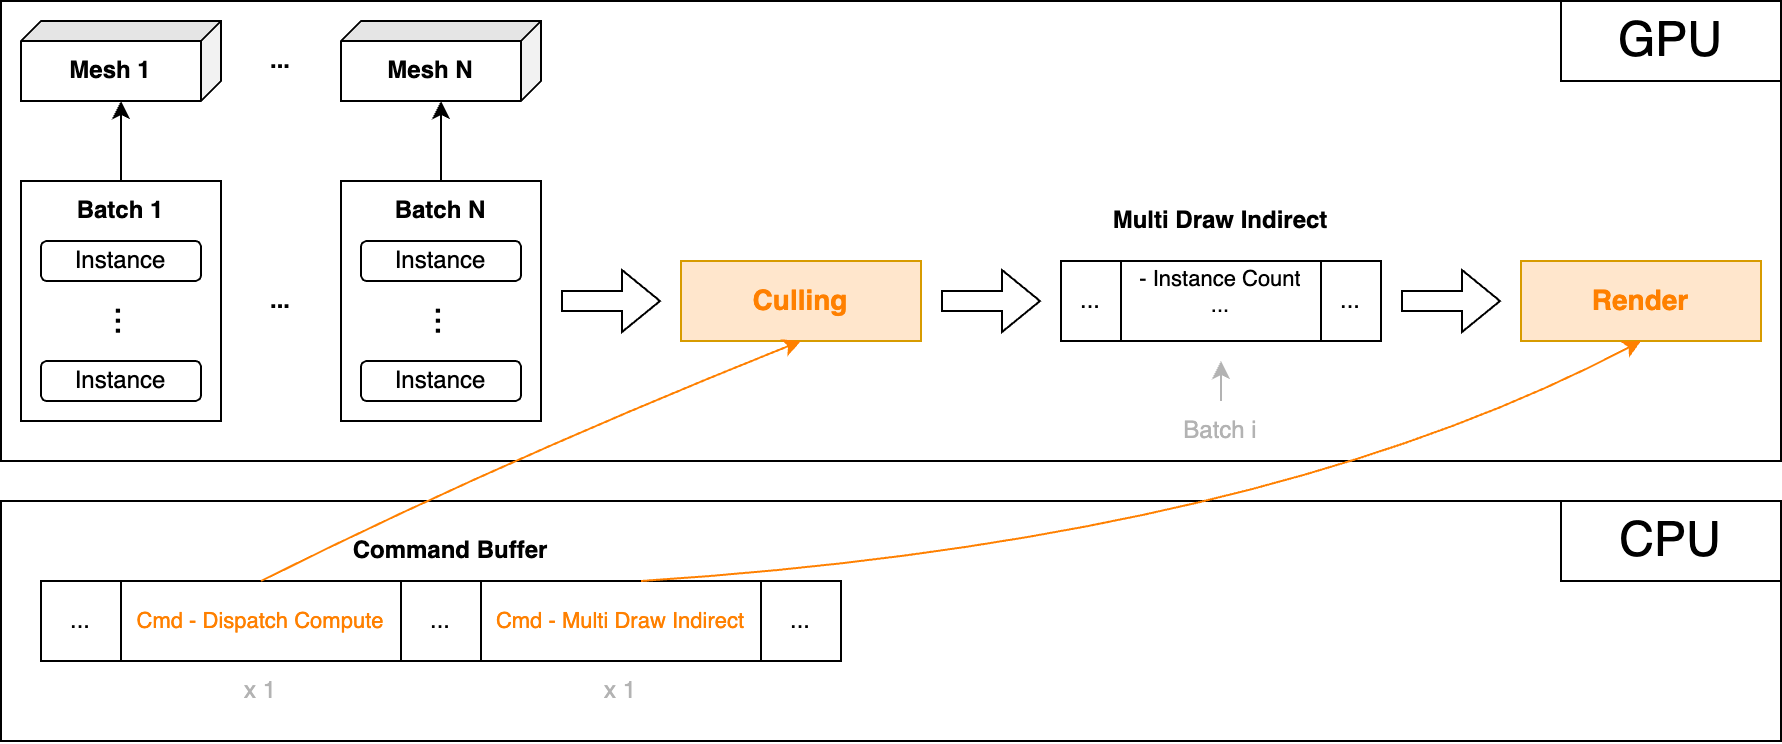
\includegraphics[scale=0.26]{renderer/meshes_render.png}
    \caption{Схема процесса рендеринга мешей.}
    \label{fig:meshes_render}
\end{figure}

При самой отрисовке используются техники физически корректного рендеринга (PBR) для достижения более визуально реалистичных результатов. PBR симулирует взаимодействие света с поверхностями в соответствии с физическими законами, что позволяет материалам выглядеть и вести себя как их реальные аналоги. Шейдерный код основан на решениях, представленных в \cite{pbr_book2016}.

\subsection{Кластерное отсечение света}
Одна из наиболее затратных (по объему необходимых вычислительных ресурсов) операций в графике является просчет освещения. Современные виртуальные сцены состоят из множества сложной геометрии и источников света. С физической точки зрения, свет, излучаемый источником света распространяется бесконечно далеко, однако в качестве вычислительной аппроксимации, учитывая что затухание света пропорционально $\frac{1}{d^2}$ (где $d$ -- расстояние от источника света), можно посчитать радиус точечного источника света, вне которого вклад будет пренебрежимо малым (см. коэффициент затухания \ref{eq:point_light_attenuation}; заметим, что $\text{Attenuation}(\text{LightRadius}) = 0$). Эта идея положила основу методам отсечения источников света \cite{Harada2012ForwardBD}, которые оптимизируют расчет освещения путем определения групп фрагментов, на которые не влияет определенный источник света.
\begin{align}
    \text{Attenuation}(d) \approx \frac{max \left(1 - \frac{d}{\text{LightRadius}}, 0\right) }{d^2}
    \label{eq:point_light_attenuation}
\end{align}

Метод кластерного отсечения света (clustered light culling) разделяет пирамиду видимости камеры на трехмерные кластеры, каждый из которых содержит информацию о всех источниках света, которые могут повлиять на пиксели в этом кластере. Кластеры расположены таким образом, что они полностью покрывают всю сцену и не пересекаются между собой. Для быстрой проверки пересечений для каждого кластера, то есть усеченной пирамиды, считается минимальный параллельный осям ограничивающий параллелепипед (англ. axis-aligned bounding box или AABB), содержащий весь объем кластера. Ограничивающий же объем для точечных источников света -- сфера.

\begin{figure}[h]
    \centering
    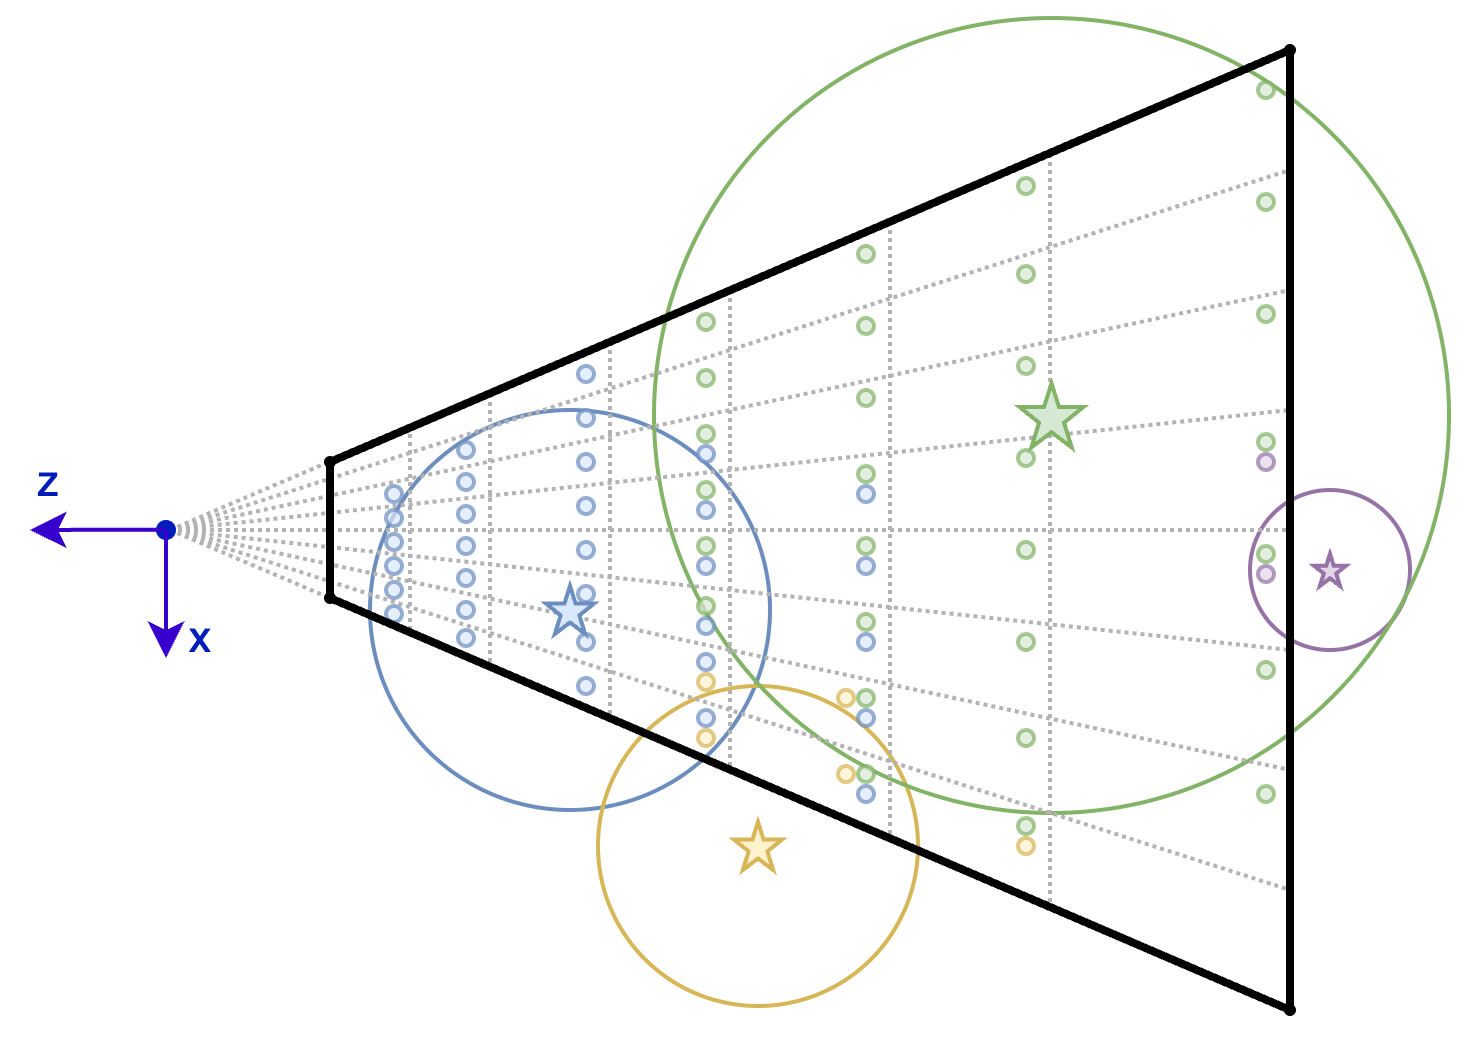
\includegraphics[scale=0.25]{renderer/clustered_light_culling_frustum_xz.png}
    \caption{Отсечение точечных источников света относительно трехмерных кластеров (вид в проекции на плоскость X-Z)}
    \label{fig:clustered_light_culling_frustum_xz}
\end{figure}

Существует несколько способов разбиения на кластеры. Дальше представлено разбиение, основанное на работе \cite{original_clustered_light_culling}. В плоскости X-Y экран разбивается равномерно на ячейки одинакового размера (в данной работе -- 16x16 пикселей). По глубине (вдоль оси Z) же пирамида разделяется экспоненциально, однако была выбрана более простая вычислительно аппроксимация разделения, представленная в докладе \cite{doom_clustered_z_splitting}:
\begin{align}
    z = \text{Near} \cdot \left( \frac{\text{Far}}{\text{Near}} \right) ^ {\text{SliceIndex} / \text{NumSlices}}
\end{align}

Данный алгоритм работает в два этапа -- построение ограничивающих объемов кластеров и непосредственное отсечение света. Первый шаг достаточно выполнять лишь при изменении размеров экрана, то есть когда пирамида видимости изменяется по форме. Второй шаг необходимо выполнять каждый раз когда изменяется положение и/или ориентация камеры, а также при движении источников света. Поскольку в современных видеоиграх преобладает непрерывная динамичность, на практике отсечение света вычисляется каждый кадр. Вызов вычислительного шейдера производится по количеству кластеров по соответствующим трехмерным индексам, то есть одна рабочая группа соответствует одному кластеру. Внутри рабочей группы каждый поток проверяет пересечения данного кластера с $\frac{\text{NumLights}}{\text{WorkGroupSize}}$ источниками света. По итогу внутри рабочей группы соберется полный список источников света (а точнее их индексов, для сокращения необходимой алгоритму видеопамяти), влияющих на данный кластер. Дальше этот список переносится из shared memory в глобальный буфер, который в последствии будет использоваться при подсчете освещения.

Помимо самого алгоритма, также была реализована отладочная визуализация комплексности освещения, которая отображается поверх просчитанного изображения. На каждый фрагмент добавляется цвет, показывающий как много источников света было обработано в расчете освещения данного фрагмента. Эта визуализация полезна не только для отладки работы представленного алгоритма, но также и для работы дизайнеров сцен, которые могут благодаря ней оптимизировать расстановку источников света, избегая большого количества пересечений источников света.

\subsection{Симуляция и отрисовка частиц}
Системы частиц являются важным компонентом компьютерной графики, используемым для моделирования таких явлений, как огонь, дым, дождь, взрывы и др. Традиционно эти системы обрабатывались на центральном процессоре \cite{lucasfilm_particle_systems_1983}. Это включало вычисление позиции, скорости и других свойств каждой частицы в системе для каждого кадра. CPU выполнял все необходимые физические расчеты, включая силы, такие как гравитация, ветер и столкновения. Однако ранние реализации систем частиц были вынуждены использовать упрощенную физику, методы рендеринга и малое количество частиц для достижения желаемых визуальных эффектов в рамках ограничений вычислительной мощности CPU, поскольку CPU не предназначены для высокопараллельной природы симуляций. Появление вычислительных шейдеров привело к переносу значительной части этой работы на GPU.

Симуляция частиц использует параллельную архитектуру GPU для обработки всего жизненного цикла частиц, от их "рождения" до "смерти". Подробная диаграмма системы частиц изображена на рисунке \ref{fig:particle_system_simulation_and_render}. Алгоритм разбит на три части:
\begin{enumerate}
    \item Emission (инициализация): в вычислительном шейдере "излучаются" новые частицы и инициализируются их атрибуты, такие как положение, скорость, цвет и время жизни. Поскольку на GPU нет динамических массивов, используется один буфер фиксированного размера со всеми частицами. Для определения, какие элементы (частицы) этого буфера свободны, используется вспомогательный буфер -- free list.
    \item Simulation (симуляция): каждый кадр другой вычислительный шейдер обновляет атрибуты частиц на основе физических расчетов. Это может включать применение сил, обновление скоростей и проверку на столкновения. В случае, если время жизни частицы закончилось, ее индекс добавляется в free list. Также, на этом этапе происходит запись индексов действующих и видимых частиц в еще один вспомогательный буфер.
    \item Rendering (отрисовка): как и при отрисовке мешей здесь используется метод GPU-driven rendering. Этап симуляции генерирует команду отрисовки на GPU, где instance count равен числу действующих и видимых частиц. В качестве геометрии для отрисовки используются четырехугольники, ориентированные в сторону камеры \cite{schaufler1995dynamically}, на которые потенциально накладывается текстурный атлас (по времени жизни выбирается текущая текстура).
\end{enumerate}

\begin{figure}[h]
    \centering
    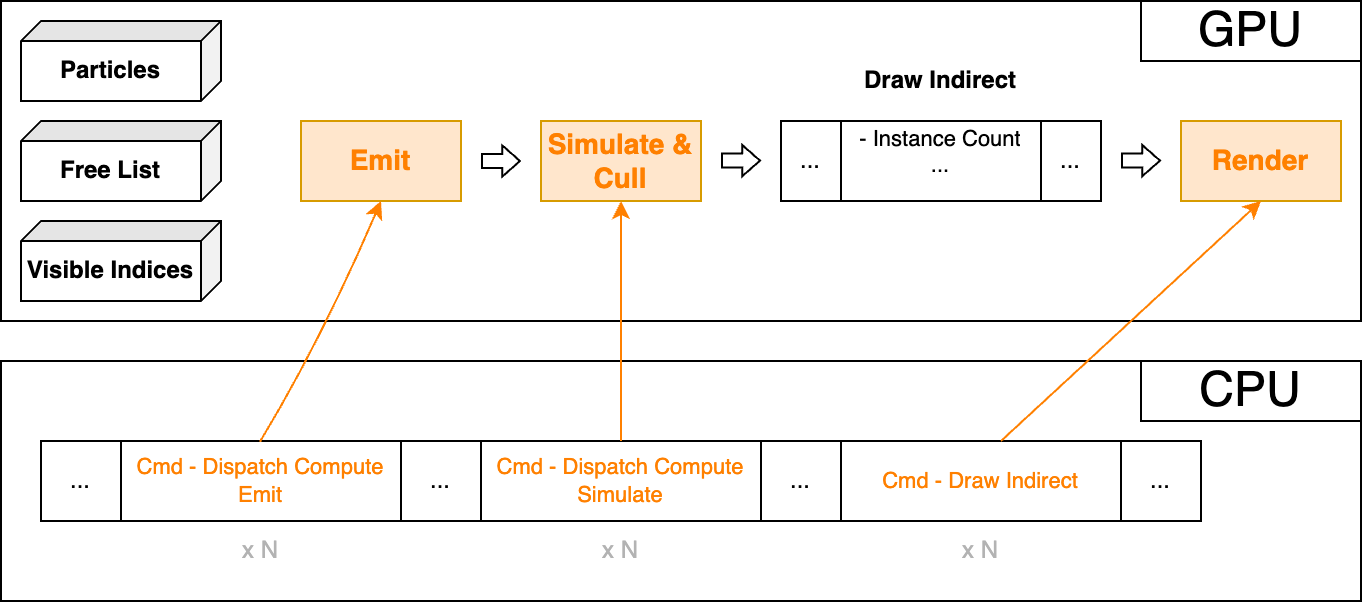
\includegraphics[scale=0.3]{renderer/particle_system_simulation_and_render.png}
    \caption{Схема процесса симуляции и рендеринга частиц}
    \label{fig:particle_system_simulation_and_render}
\end{figure}

\subsection{Эффекты постобработки}
Следующим концептуально отличающимся элементом рендерера является стек эффектов постобработки. Данные эффекты преобразуют уже отрендеренное изображение. В данной работе были реализованы два эффекта -- bloom и tone mapping.

\subsubsection{Bloom}
Эффект свечения (bloom) является популярной техникой постобработки, используемой для имитации рассеивания яркого света в человеческом глазу, создавая светящийся ореол вокруг ярких областей изображения. Этот эффект улучшает реалистичность сцен, особенно тех, которые включают интенсивные источники света, такие как солнце, огни или отражающие поверхности. Для данного эффекта необходимо, чтобы входное изображение было с высоким динамическим диапазоном (HDR), где контраст между яркими и темными областями более выражен.

Алгоритм генерации данного эффекта был взят из доклада \cite{cod_aw_bloom} и состоит из сначала последовательного downsampling, используя кастомный фильтр (см. рисунок \ref{fig:bloom_downsample}), который был придуман для борьбы с негативными темпоральными артефактами, а потом последовательного аддитивного upsampling с тент-фильтром размера 3x3 (см. формулу \ref{eq:tent3x3}) и композиции. Схематично этапы работы алгоритма представлены на рисунке \ref{fig:bloom_diagram}.

\begin{align}
    \text{T} = \frac{1}{16} \begin{bmatrix}
                                1 & 2 & 1 \\[0.1em]
                                2 & 4 & 2 \\[0.1em]
                                1 & 2 & 1
                            \end{bmatrix} \label{eq:tent3x3}
\end{align}

\begin{figure}[h]
    \centering
    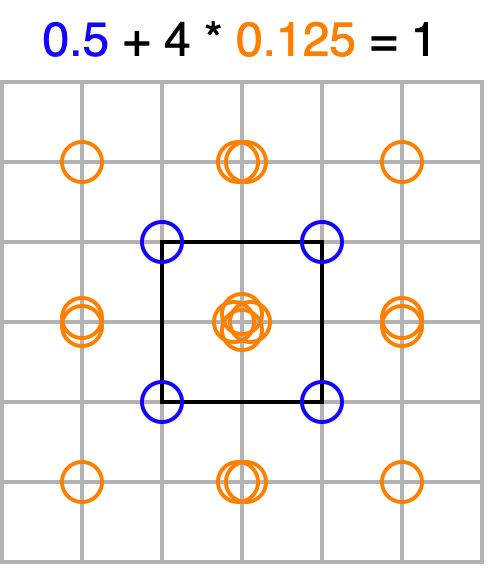
\includegraphics[scale=0.26]{renderer/bloom_downsample.png}
    \caption{Кастомный downsample, митигирующий негативные темпоральные артефакты.}
    \label{fig:bloom_downsample}
\end{figure}

\begin{figure}[h]
    \centering
    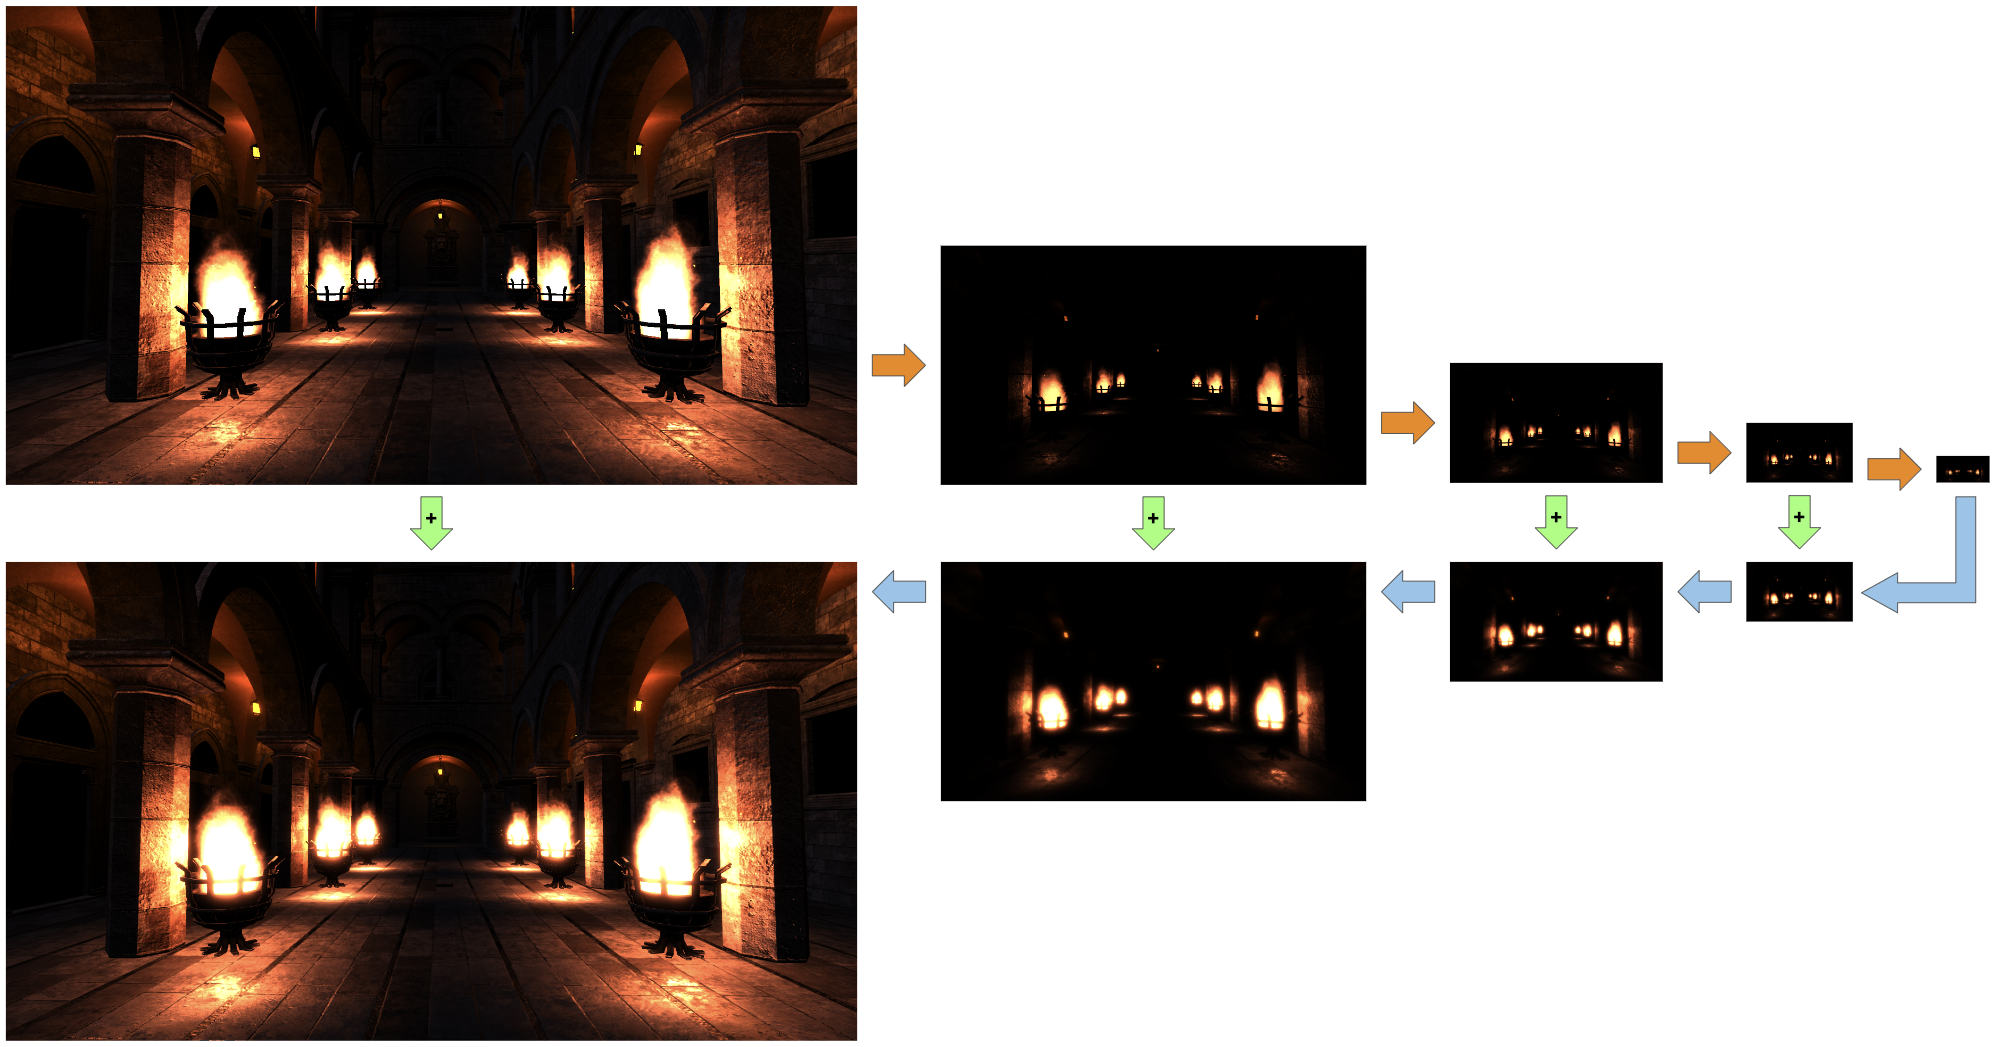
\includegraphics[scale=0.23]{renderer/bloom_diagram.png}
    \caption{Схема просчета эффекта свечения. Изображения представлены без применения tone mapping.}
    \label{fig:bloom_diagram}
\end{figure}

Первый downsampling отличается от последующих. На нем кастомный фильтр считается по взвешенным средним использованных семплов \cite{karis2014}, используя luma: $w(L_\text{HDR}) = \frac{1}{1 + \text{luma}\left( L_\text{HDR} \right)}$, где $\text{luma}\left( v \right) = dot\left( (0.2126, 0.7152, 0.0722), v^{-2.2} \right)$, а после этого происходит отделение только "ярких" частей, что сделано для возможности художественной конфигурации эффекта при помощи параметров $t$ (\textit{threshold}) и $s$ (\textit{soft threshold}):

\begin{align}
    B( c ) &= max( c.r, c.g, c.b ) & \text{яркость}&\\
    S( c ) &= \frac{ ( clamp( B( c ) - t + t s,  0,  2 t s ) )^2 }{ 4 \cdot (t s + bias) } & \text{смягчающая кривая}&\\
    P( c ) &= c \cdot \frac{ max( S (B(c)), B(c) - t ) }{max(B(c), bias)} & \text{результат префильтрации}\label{eq:bloom_prefilter_config}
\end{align}

\subsubsection{Tone mapping}
Тональное отображение (англ. tone mapping) является ключевым процессом в рендеринге с высоким динамическим диапазоном (HDR), позволяющим преобразовать изображения, которые имеют широкий диапазон значений яркости, в формат, подходящий для отображения на стандартных дисплеях с ограниченным динамическим диапазоном. В данной работе реализовано тональное отображение на основе экспозиции \cite{tone_mapping}, динамически регулирующее экспозицию различных областей изображения для сохранения деталей по всему спектру яркости, обеспечивая видимость и правильное отображение как теней, так и высветлений (см. рисунки \ref{fig:tone_map_vis}). Формула отображения представлена ниже:
\begin{align}
    L_{\text{mapped}}(x, y) = \left( 1, 1, 1 \right) - e^{-L_{\text{HDR}}(x, y) \cdot \text{exposure}}
\end{align}

\begin{figure}[h]
    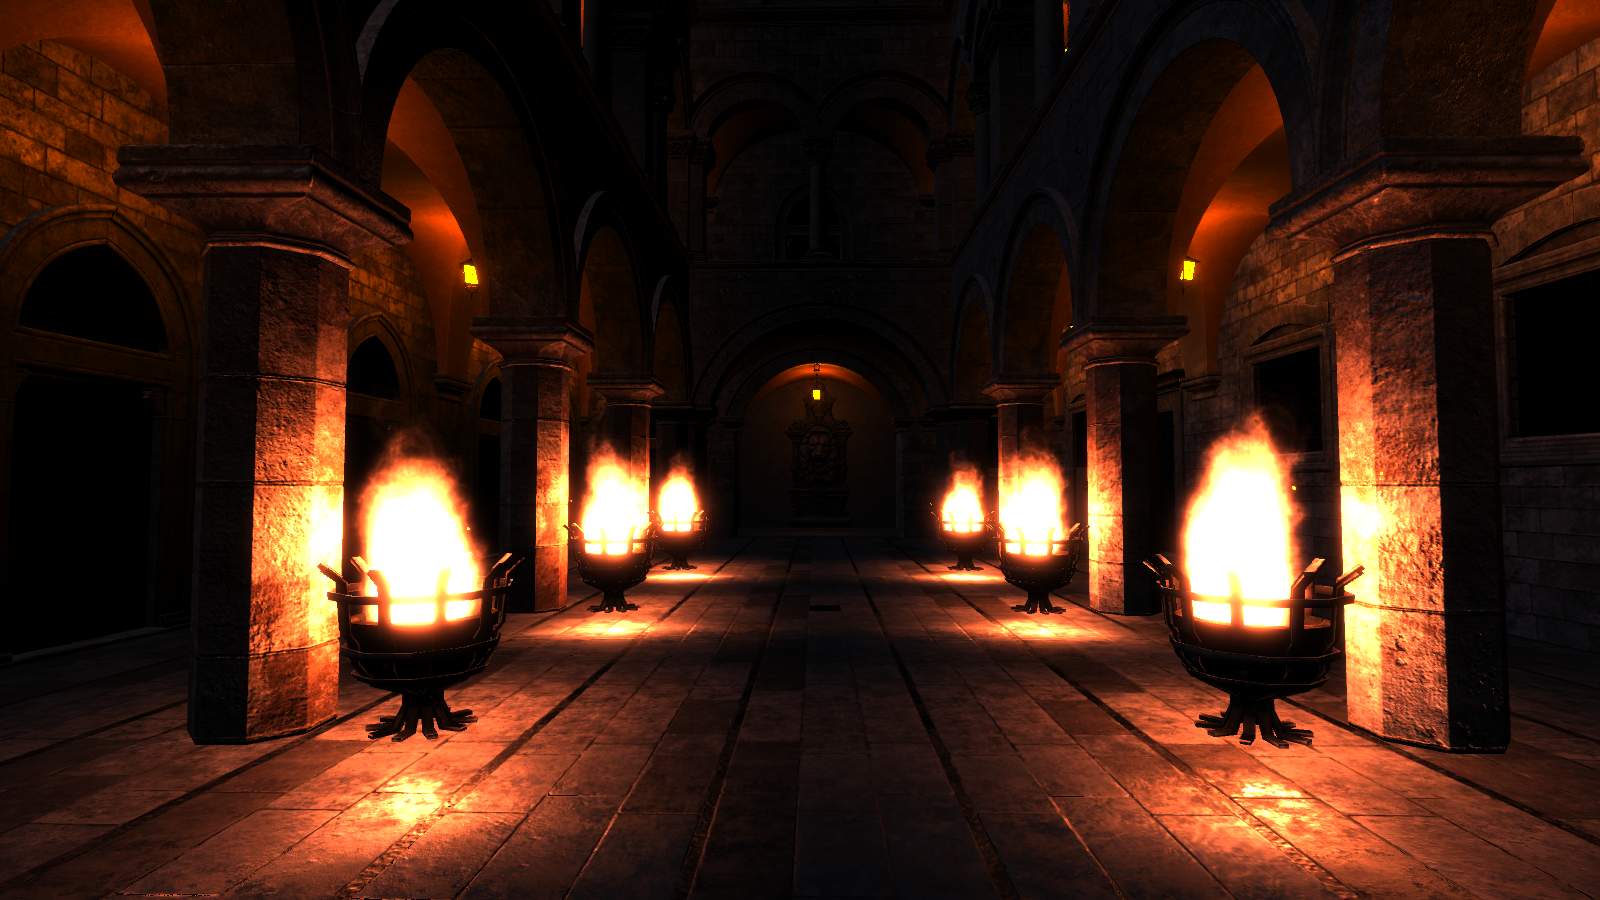
\includegraphics[scale=0.145]{renderer/pre_tonemap.png}
    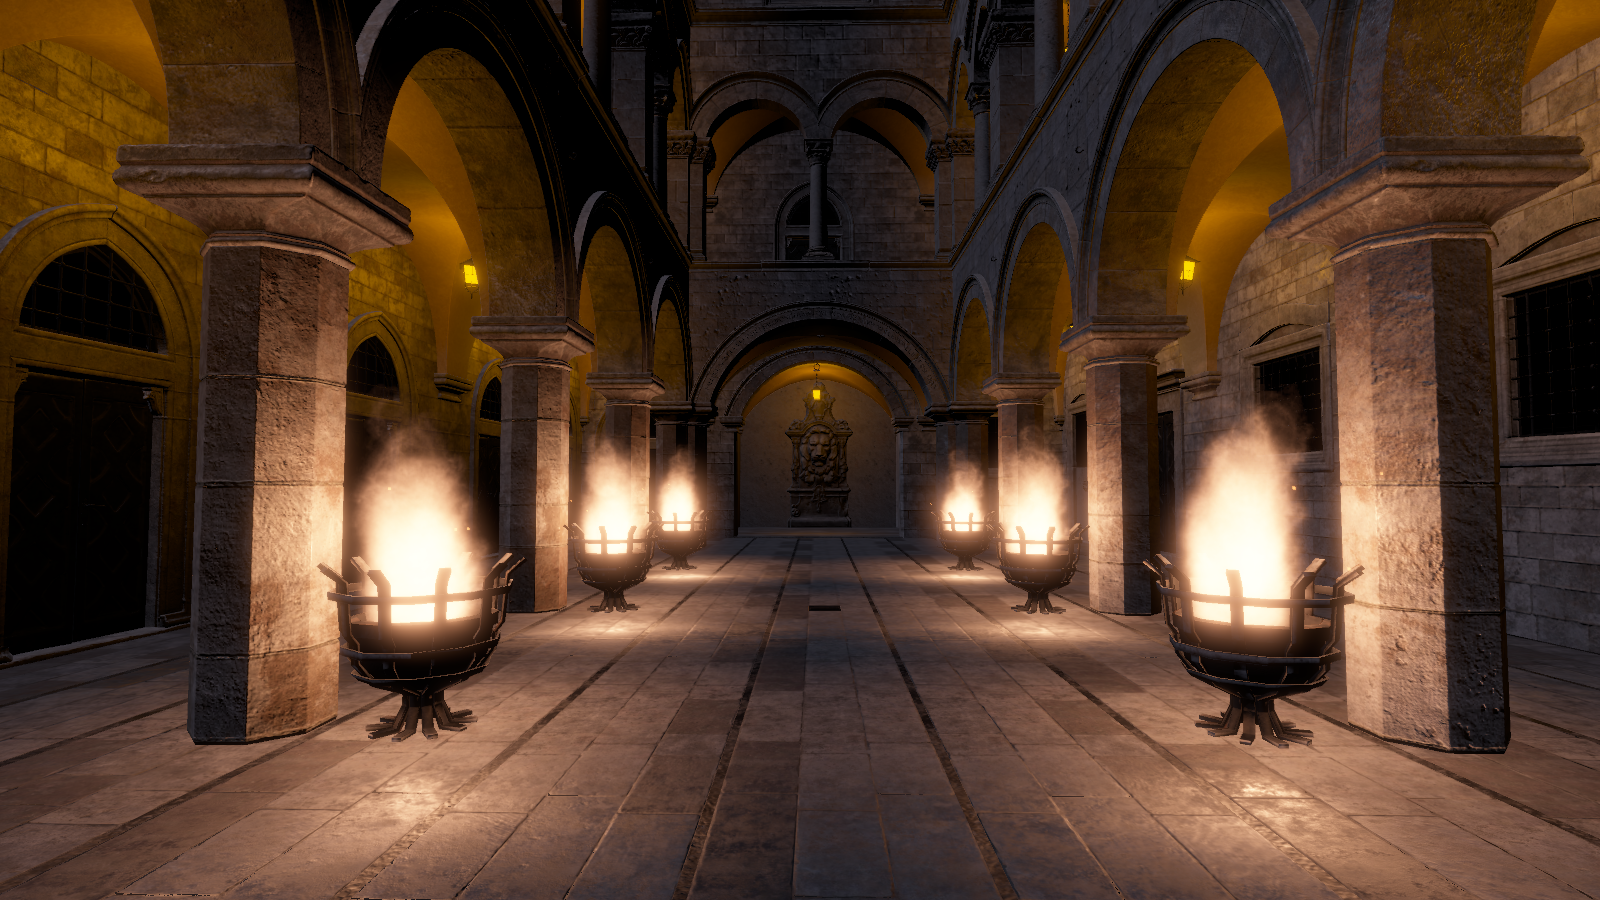
\includegraphics[scale=0.145]{renderer/post_tonemap.png}
    \caption{Визуализация тонального отображения с $\text{exposure} = 0.6$; слева направо: $L_{\text{HDR}}(x, y)$ и $L_{\text{mapped}}(x, y)$.}
    \label{fig:tone_map_vis}
\end{figure}


\newpage
\section{Результаты}
Имплементация описанного выше решения была написана на C++20 с использованием библиотек Assimp, EnTT, fmt, GLFW, GLM, glslang, magic-enum, stb-image, taskflow, VMA, volk, yaml-cpp. Исходный код имеет размер порядка 12 000 строк (не учитывая шейдерный код) и доступен по ссылке \url{https://github.com/tralf-strues/liger-engine}. В качестве тестовых моделей были выбраны сцена Sponza Atrium \cite{sponza_atrium} и меш Medieval Brazier \cite{medieval_brazier} с максимально возможным разрешением текстур.

В следующей таблице приведен анализ одного кадра тестового приложения. Замеры были произведены на компьютере с центральным процессором Intel Core i7-9750H (2.6Ghz) и видеокартой NVIDIA GeForce GTX 1660 Ti (Max-Q Design) при разрешении изображения 1920x1080 пикселей и MSAAx8. Для получения метрик использовался профилировщик NVIDIA Nsight Graphics \cite{nsight}.

\begin{table}[ht]
    \centering
    \begin{tabular}{ p{70mm} | p{30mm} }
    \textbf{Показатель} & \textbf{Значение} \\
    \hline
    \hline
    Меши: instances total & 115 \\
    Меши: instances passed culling & 81 \\
    Меши: triangles total & 3 781 554 \\
    Меши: triangles passed culling & 3 318 486 \\
    \hline
    Кол-во источников света & 28 \\
    Сред. кол-во источников / кластер & 1.53 \\
    Макс. кол-во источников / кластер & 6 \\
    \hline
    \hline
    Clustered Light Cull время & 0.9 мс \\
    \hline
    Particle Emit время & 0.1 мс \\
    Particle Update время & 0.12 мс \\
    Particle Render время & 0.12 мс \\
    \hline
    Mesh Frustum Cull время & <0.01 мс \\
    Mesh Render время & 3.11 мс \\
    \hline
    Bloom время & 0.4 мс \\
    Tone mapping время & 0.07 мс \\
    \hline
    \hline
    Время кадра, мс & 5.2 мс \\
    FPS (кадры в секунду) & 192 \\
    \end{tabular}
    \caption{Анализ одного кадра исполнения тестового приложения.}
    \label{tbl:frame_stats}
\end{table}

Визуализация (без подробной информации, такой как барьеры и параметры ресурсов) кадрового графа реализованного рендерера, сгенерированная собственным отладочным модулем, представлена на рисунке \ref{fig:res_rg_basic}. Более детальная визуализации слишком большая для размещения в данной работе.

\begin{figure}[h]
    \centering
    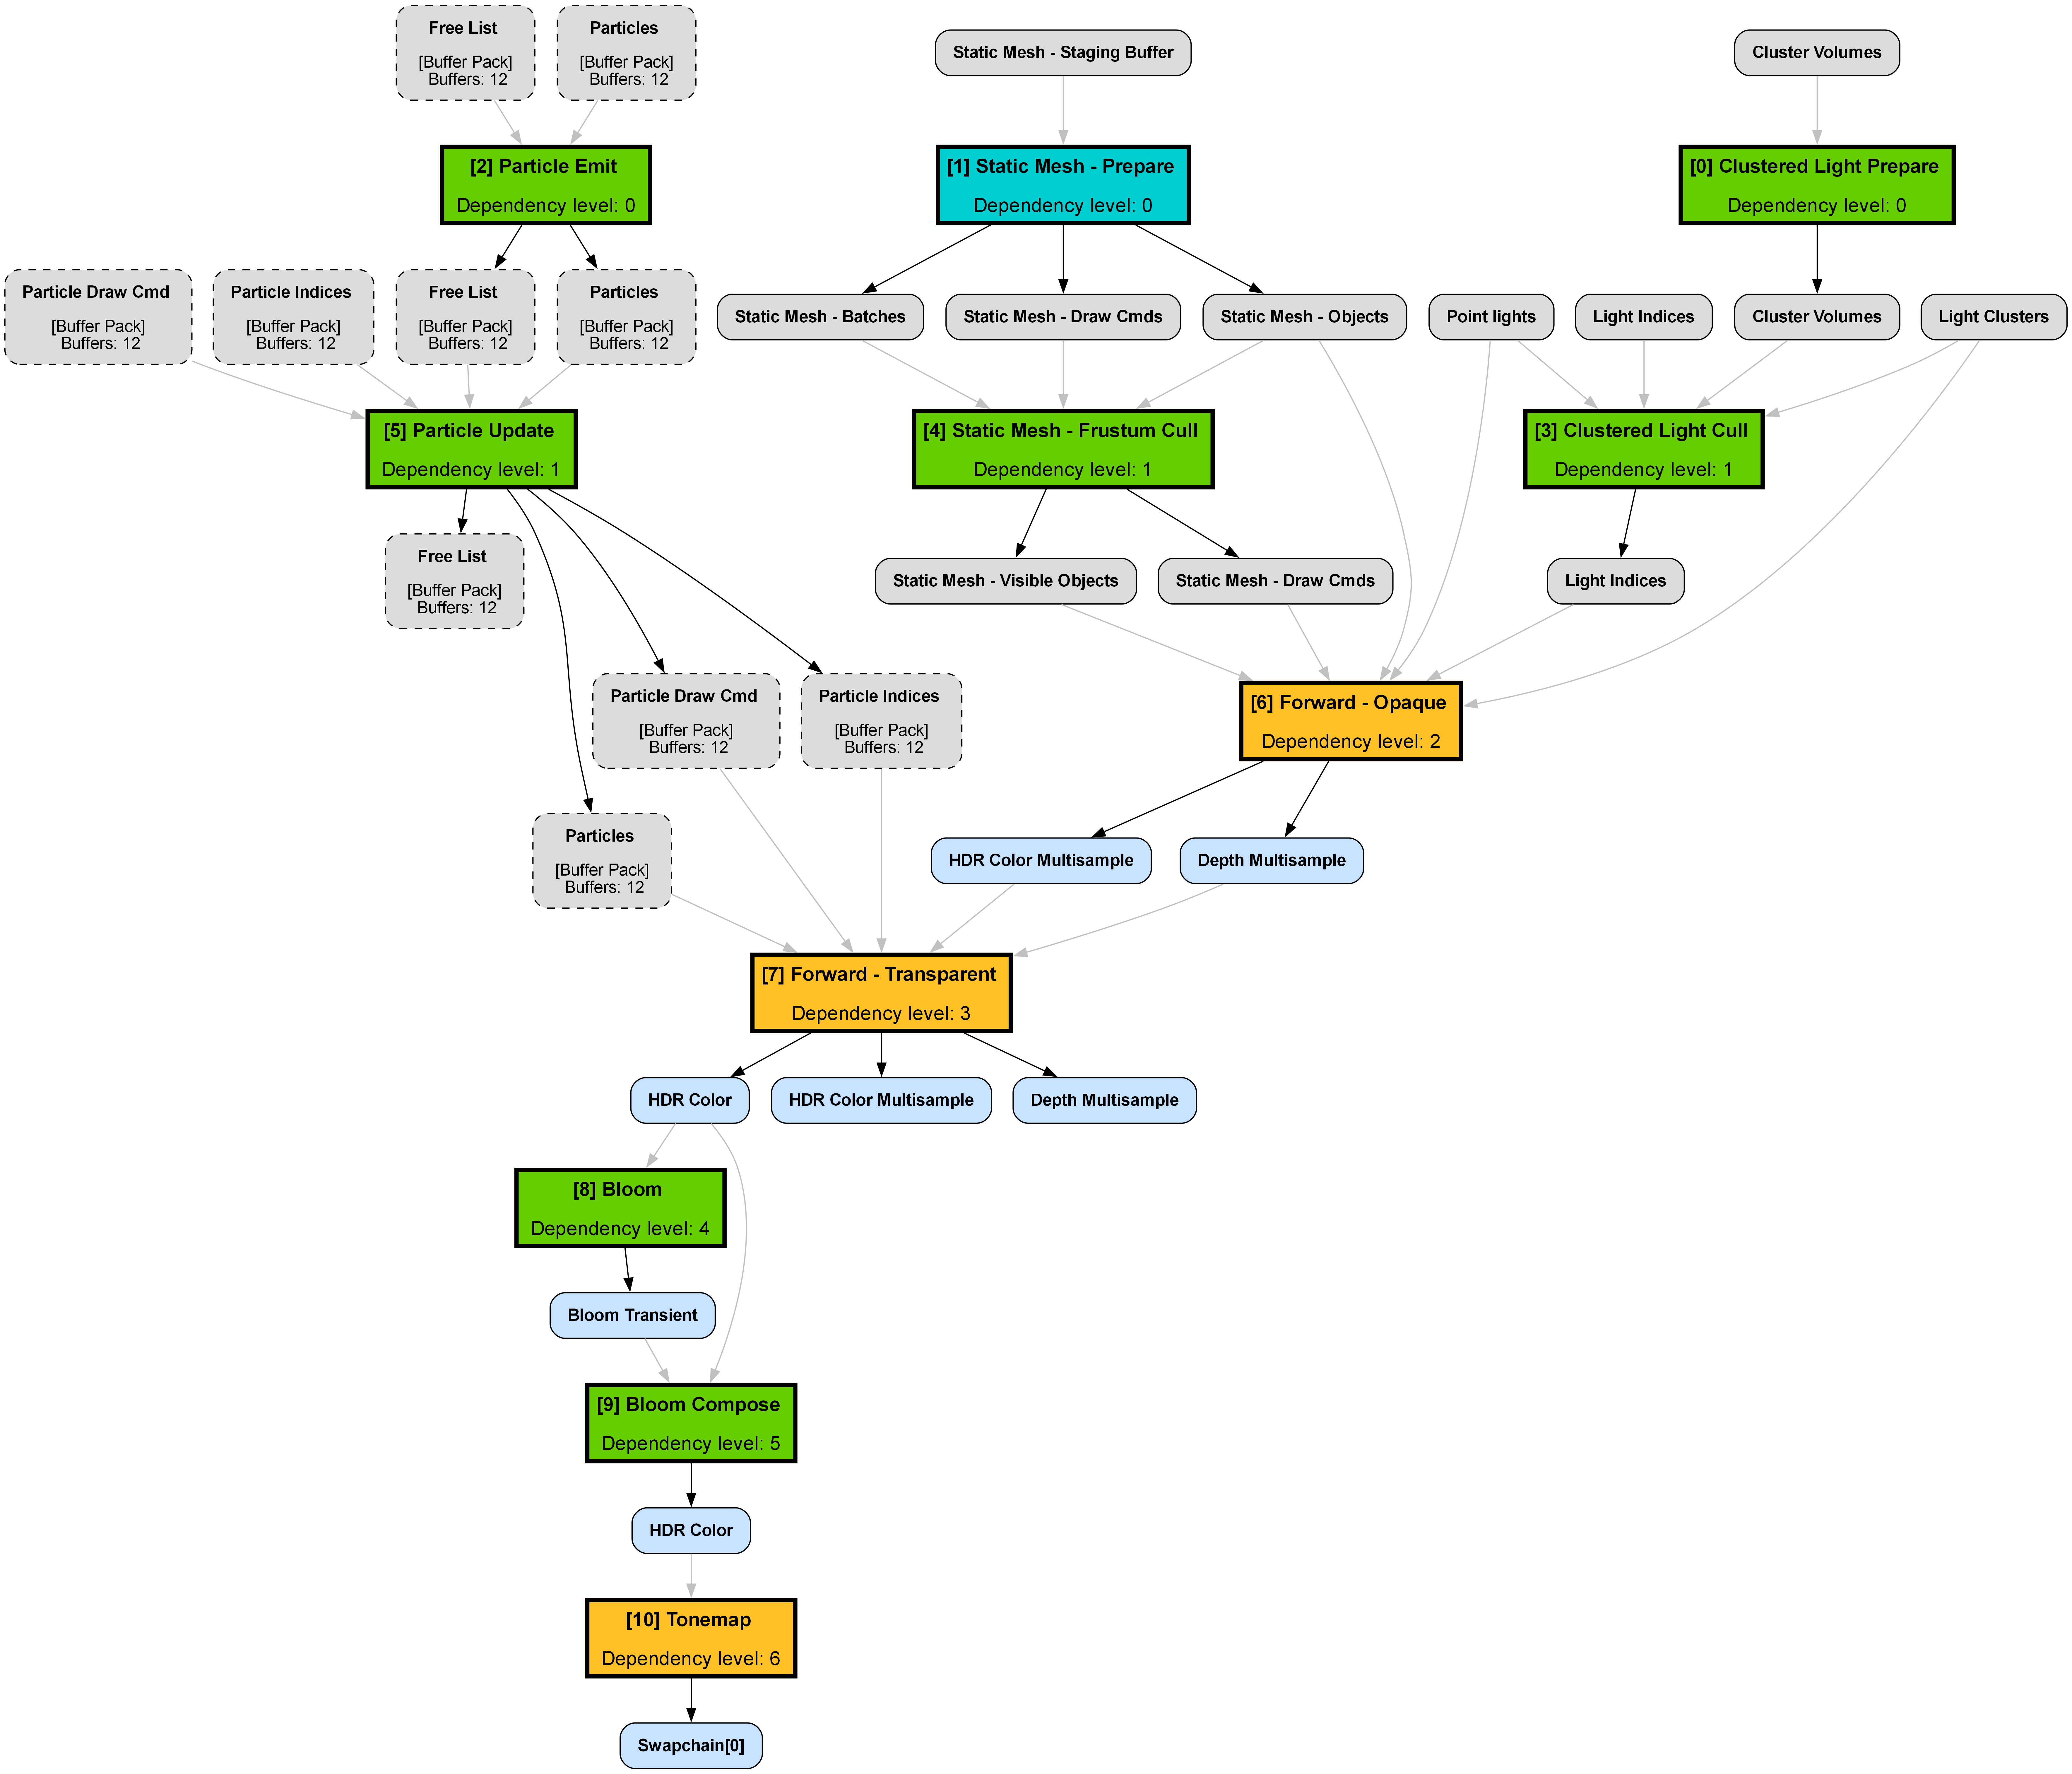
\includegraphics[scale=0.066]{renderer/rg_basic.png}
    \caption{Кадровый граф рендерера, представленного в данной работе.}
    \label{fig:res_rg_basic}
\end{figure}
\newpage
\section{Заключение}
В рамках проведенной работы были уточнены детали устройства метода рендеринга с использованием кадровых графов, написана реализация кадрового графа с поддержкой нескольких командных очередей, предложен ряд новых архитектурных решений в проектировании Render Hardware Interface, а также написан рендерер, использующий современные подходы к графике, такие как вычислительные шейдеры и gpu-driven rendering, в качестве доказательства валидности нового дизайна.

В силу комплексности современных графических API, при дальнейших исследованиях планируется повышать производительность и качество алгоритма планировки задач кадрового графа. Планируется реализовать оптимизированную имплементацию компиляции в случае использования только одной или двух очередей, поскольку в таком случае сложность сильно понижается и нет необходимости рассматривать некоторые сценарии, ввиду их невозможности.

Еще одним крупным направлением для дальнейших исследований является написание фронтенда декларации графов в данных. Это может быть как интеграция в систему шейдеров (как это сделано в \cite{amd_rps_sdk}), так и построение с помощью визуального редактора узлов, подобно современным редакторам игровых скриптов или материалов \cite{material_editor_ue5}.

Подход интеграции кадровых графов в RHI весьма перспективен в применении к современным приложениям реального времени, поскольку на данном низком уровне абстракции держится весь высокоуровневый рендеринг, который становится все более комплексным с каждым годом. Данный подход позволит более эффективно использовать ресурсы GPU, позволяя графическим разработчикам концентрироваться на совершенствовании отдельных графических эффектов, делегируя связи и планировку кадровым графам, а поэтому данный подход заслуживает дальнейшего исследования и усовершенствования.
\newpage
\printbibliography
%%%%%%%%%%%%%%%%%%%%%%%%%%%%%%%%%%%%%%%%%%%%%%%%%%%%%%%%%%%%%%%%%%%%%%%%%%%%%%%%
\end{document}
